\chapter{Fourier变换}
\label{chap:fourier-transform}
\label{chap:orthogonal-expansions-transforms}

一段周期振动可以看成若干个频率的叠加：基频决定音高，各次谐波的强弱决定音色。把函数写成复指数$e^{\mathrm ikx}$的组合，就是为它换上一套频率坐标。在这套坐标下，平移变成乘一个相位因子，求导变成乘频率，卷积变成逐频率相乘，许多在原变量下要做积分的运算化为乘法。问题在于这套坐标对哪些函数有意义、在什么意义下能把函数还原，以及那些运算规则在什么条件下成立。

本章先处理周期函数。第~\ref{sec:fourier-series}节在周期区间上用复指数正交系读出Fourier系数，由完备性得到$L^2$中的展开，再分别核对逐点收敛与一致收敛需要的额外正则性。非周期函数没有离散的谐波，频率要取遍整个实轴，求和变为积分。第~\ref{sec:fourier-l1}节对绝对可积函数定义Fourier变换，研究它的有界性、连续性与高频衰减，再单独回答反演何时成立。

$L^1$中的积分定义有一个缺陷：平方可积的函数未必绝对可积，而能量关系天然属于$L^2$。第~\ref{sec:fourier-l2}节用截断与稠密延拓把变换推广到$L^2$，得到保持范数与内积的反演。第~\ref{sec:fourier-operations}节在固定的函数空间中推导平移、缩放、微分与卷积的变换规则。第~\ref{sec:fourier-discrete}节比较连续频率、周期系数与有限维离散变换这三种表示，说明它们之间的转换需要周期化或取样。

全章固定归一化：周期取$2\pi$，系数带因子$1/(2\pi)$；全空间变换的指数取$e^{-2\pi\mathrm ix\cdot\xi}$，这样反演与能量关系中不出现额外常数。有限项截断或频带截断的逼近误差统一在第~\ref{chap:function-approximation}章研究；用尺度与位置同时组织局部细节的表示，是第~\ref{chap:wavelet-transform}章的小波变换。

\section{Fourier级数}
\label{sec:fourier-series}

在$\mathbb R^n$中取一组标准正交基$q_1,\ldots,q_n$，向量$v$的第$j$个坐标就是内积$a_j=\langle q_j,v\rangle$，并且$v=\sum_ja_jq_j$，$\lVert v\rVert^2=\sum_j\lvert a_j\rvert^2$。第~\ref{chap:function-inner-product-spaces}章把这套做法搬到了Hilbert空间。本节把它用在周期函数上，基取复指数$e^{\mathrm ikx}$，第$k$个基函数在一个周期内恰好转$k$圈，所以坐标记录的是第$k$次振荡的强弱。

先在$L^2$中建立展开，这是类比最直接的部分。然后问部分和在每一点、或在整个周期上一致地趋于什么，这两个问题要用到正交性之外的条件。

\subsection{\texorpdfstring{$L^2$}{L2}中的Fourier展开}
\label{sec:fourier-series-l2}

\paragraph{周期函数与归一化内积}

本节的函数都以$2\pi$为周期。等价地，可以把它看成区间$[-\pi,\pi)$上的函数，并把两个端点粘成一点。记这样的周期区间为$\mathbb T$，积分都在一个周期上进行。平方可积的周期函数组成$L^2(\mathbb T)$，它的元素是几乎处处相等的函数组成的等价类，第~\ref{chap:function-inner-product-spaces}章已证明它是Hilbert空间。

沿用第~\ref{chap:function-inner-product-spaces}章的约定，内积对第二个变量线性。我们在内积前放一个因子$1/(2\pi)$，使常数函数$1$的长度恰好为$1$：
\begin{equation}
\langle f,g\rangle=\frac1{2\pi}\int_{-\pi}^{\pi}\overline{f(x)}\,g(x)\,\mathrm dx .
\label{eq:fourier-circle-inner-product}
\end{equation}
相应的范数是$\lVert f\rVert_2=\langle f,f\rangle^{1/2}$。同样地，$L^1$范数也取平均：
\[
\lVert f\rVert_1=\frac1{2\pi}\int_{-\pi}^{\pi}\lvert f(x)\rvert\,\mathrm dx.
\]

记$e_k(x)=e^{\mathrm ikx}$，$k\in\mathbb Z$。下面验证它们标准正交。当$k=j$时，被积函数恒为$1$，所以$\langle e_j,e_k\rangle=1$。当$k\neq j$时，令$m=k-j\neq0$，直接积分得到
\[
\langle e_j,e_k\rangle=\frac1{2\pi}\int_{-\pi}^{\pi}e^{\mathrm imx}\,\mathrm dx
=\frac{e^{\mathrm im\pi}-e^{-\mathrm im\pi}}{2\pi\mathrm im}.
\]
由于$e^{\mathrm imx}$以$2\pi$为周期，分子中两个端点的值相同，所以
\[
\langle e_j,e_k\rangle=0.
\]
这正是周期性的作用：一个整数圈的旋转，正负部分恰好抵消。

\paragraph{Fourier系数与部分和}

有了标准正交系，第$k$个坐标自然就是与$e_k$的内积。

\begin{definition}[Fourier系数与Fourier级数]
\label{def:fourier-coefficients}
对$f\in L^1(\mathbb T)$，称
\begin{equation}
\widehat f(k)=\frac1{2\pi}\int_{-\pi}^{\pi}f(x)e^{-\mathrm ikx}\,\mathrm dx ,\qquad k\in\mathbb Z
\label{eq:fourier-coefficient}
\end{equation}
为$f$在方向$e_k$上的坐标，称为第$k$个\term{Fourier系数}（Fourier coefficient）。形式级数$\sum_{k\in\mathbb Z}\widehat f(k)e^{\mathrm ikx}$称为$f$的\term{Fourier级数}（Fourier series），它的对称部分和记为
\begin{equation}
S_Nf=\sum_{\lvert k\rvert\leq N}\widehat f(k)\,e_k .
\label{eq:fourier-partial-sum}
\end{equation}
\end{definition}

对$f\in L^2(\mathbb T)$，式~\eqref{eq:fourier-coefficient}就是$\widehat f(k)=\langle e_k,f\rangle$。只要$f$可积，系数就有定义，并且$\lvert\widehat f(k)\rvert\leq\lVert f\rVert_1$。一个周期的长度有限，由Cauchy--Schwarz不等式，$L^2(\mathbb T)\subseteq L^1(\mathbb T)$，所以平方可积函数都有系数。

于是一个函数对应一列坐标$[\ldots,\widehat f(-1),\widehat f(0),\widehat f(1),\ldots]$。下面算一个完整的例子，后面的定理都会回到它。

\begin{example}[方波的坐标]
\label{ex:fourier-square-wave}
取方波：在$(0,\pi)$上$f=1$，在$(-\pi,0)$上$f=-1$，再按$2\pi$周期延拓；在$0$和$\pm\pi$处的取值暂不规定。

$f$是奇函数，所以$\widehat f(0)=0$。对$k\neq0$，把积分分成两段：
\[
\widehat f(k)=\frac1{2\pi}\Bigl(\int_0^{\pi}e^{-\mathrm ikx}\,\mathrm dx-\int_{-\pi}^0e^{-\mathrm ikx}\,\mathrm dx\Bigr).
\]
两段分别积分，并用$e^{\pm\mathrm ik\pi}=(-1)^k$，得到
\[
\int_0^{\pi}e^{-\mathrm ikx}\,\mathrm dx=\frac{1-(-1)^k}{\mathrm ik},\qquad
\int_{-\pi}^0e^{-\mathrm ikx}\,\mathrm dx=\frac{(-1)^k-1}{\mathrm ik}.
\]
代回去，第$k$个系数是
\[
\widehat f(k)=\frac{1-(-1)^k}{\pi\mathrm ik}.
\]
偶数$k$的系数为零，奇数$k$的系数为$2/(\pi\mathrm ik)$，模长为$2/(\pi\lvert k\rvert)$。

把$\pm k$两项配对，括号里出现$2\mathrm i\sin kx$，得到第$k$次（$k$为正奇数）的实形式
\[
\widehat f(k)e^{\mathrm ikx}+\widehat f(-k)e^{-\mathrm ikx}=\frac4{\pi k}\sin kx.
\]
所以前几项是
\[
S_5f(x)=\frac4\pi\Bigl(\sin x+\frac13\sin3x+\frac15\sin5x\Bigr).
\]
\end{example}

图~\ref{fig:fourier-square-coordinates}把这个例子的两种“一列数”并排放在一起。左边是取值，下标是$x$；右边是坐标，下标是$k$。同一个向量换了一组基来记录，三条灰色的正弦波叠加起来，已经勾出方波的轮廓。

\begin{BookInlineFigure}
  \centering
  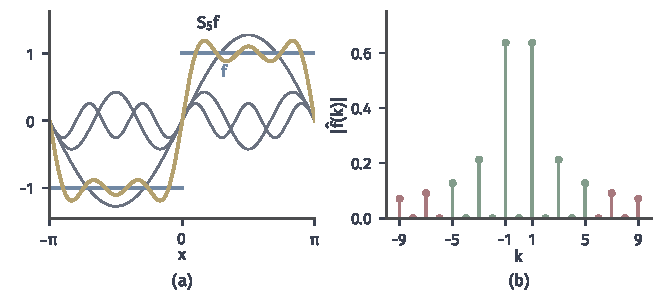
\includegraphics[width=112mm]{figures/04-spaces-measures-and-geometry/03-function-spaces/matplotlib/fourier-square-coordinates/figure.pdf}
  \caption{方波的两种记录方式。(a)蓝色为方波$f$，灰色为$\frac4{\pi}\sin x$、$\frac4{3\pi}\sin3x$、$\frac4{5\pi}\sin5x$三个分量，黄色为它们的和$S_5f$。(b)模长$\lvert\widehat f(k)\rvert$，绿色为$S_5f$保留的坐标（$\lvert k\rvert\leq5$），红色为舍弃的坐标；偶数下标的坐标都是零。}
  \label{fig:fourier-square-coordinates}
\end{BookInlineFigure}

部分和有明确的几何含义。有限组合$\sum_{\lvert k\rvert\leq N}c_ke_k$称为次数不超过$N$的\term{三角多项式}（trigonometric polynomial），它们组成$2N+1$维子空间$\mathcal T_N$。由第~\ref{chap:function-inner-product-spaces}章的有限截断定理，$S_Nf$是$f$在$\mathcal T_N$上的正交投影，也就是$\mathcal T_N$中离$f$最近的元素。同一章的Bessel不等式给出
\[
\sum_{k\in\mathbb Z}\lvert\widehat f(k)\rvert^2\leq\lVert f\rVert_2^2 .
\]

表~\ref{tab:fourier-dictionary}汇总了目前的对应。最后一行是类比失效的地方。

\begin{BookInlineTable}
  \centering
  \begin{tabular}{@{}ll@{}}
    \toprule
    $\mathbb C^n$与标准正交基$q_j$ & $L^2(\mathbb T)$与$e_k=e^{\mathrm ikx}$\\
    \midrule
    坐标$a_j=\langle q_j,v\rangle$ & Fourier系数$\widehat f(k)=\langle e_k,f\rangle$\\
    投影到前几个基向量 & 部分和$S_Nf$\\
    $\sum_j\lvert a_j\rvert^2\leq\lVert v\rVert^2$ & Bessel不等式\\
    $v=\sum_ja_jq_j$，有限和 & $f=\sum_k\widehat f(k)e_k$，$L^2$收敛\\
    $n$个正交向量自动成基 & 无穷多个正交元素未必成基\\
    \bottomrule
  \end{tabular}
  \caption{有限维标准正交基与复指数系的对应。}
  \label{tab:fourier-dictionary}
\end{BookInlineTable}

有限维中，$n$个标准正交向量必定张成全空间。无限维中，数量不能说明问题：从$\{e_k\}$中拿掉$e_0$，剩下的仍是无穷多个标准正交元素，但常数函数$1$与它们全部正交，再也表示不出来。所以写“级数”时还没有断言它收敛，更没有断言它等于$f$。要得到$L^2$中的等式，还需要证明这个系是完备的：与所有$e_k$正交的元素只有零。

\paragraph{Fejér平均}

要证明完备性，一种办法是把$f$写成三角多项式的极限，而这些三角多项式只依赖于$f$的Fourier系数。这样，系数全为零的函数就只能是零。先试部分和$S_Nf$本身。把系数的定义代入式~\eqref{eq:fourier-partial-sum}，交换有限和与积分，再利用周期函数平移不改变一个周期上的积分，得到
\begin{equation}
S_Nf(x)=\frac1{2\pi}\int_{-\pi}^{\pi}f(x-t)D_N(t)\,\mathrm dt ,
\label{eq:fourier-dirichlet-integral}
\end{equation}
其中
\[
D_N(t)=\sum_{\lvert k\rvert\leq N}e^{\mathrm ikt}
\]
称为\term{Dirichlet核}（Dirichlet kernel）。

$D_N$有闭式。当$t\notin2\pi\mathbb Z$时，这是一个公比为$e^{\mathrm it}$的几何级数，首项为$e^{-\mathrm iNt}$，共$2N+1$项：
\[
D_N(t)=e^{-\mathrm iNt}\,\frac{e^{\mathrm i(2N+1)t}-1}{e^{\mathrm it}-1}.
\]
分子分母同乘$e^{-\mathrm it/2}$，分母变成$2\mathrm i\sin(t/2)$，分子变成$2\mathrm i\sin\bigl((N+\tfrac12)t\bigr)$乘同一个相位，相位恰好抵消。于是
\begin{equation}
D_N(t)=\frac{\sin\bigl((N+\tfrac12)t\bigr)}{\sin(t/2)} .
\label{eq:fourier-dirichlet-closed}
\end{equation}

式~\eqref{eq:fourier-dirichlet-integral}是$f$的一种加权平均，但$D_N$的权有正有负。图~\ref{fig:fourier-kernels}(a)是$N=8$的情形，中央峰高$2N+1=17$，两侧的振荡并不随$N$增大而变小，这使得直接估计$S_Nf-f$很困难。

补救办法是取部分和的算术平均。令
\[
\sigma_Nf=\frac1{N+1}\sum_{n=0}^{N}S_nf,
\]
它对应的核是$F_N=\frac1{N+1}\sum_{n=0}^ND_n$，称为\term{Fejér核}（Fejér kernel）。这相当于把振荡的正负部分在不同的$n$之间相互抵消。

下面算$F_N$的闭式。由式~\eqref{eq:fourier-dirichlet-closed}，分子分母都乘$\sin(t/2)$，并用积化和差公式
\[
\sin\bigl((n+\tfrac12)t\bigr)\sin(t/2)=\tfrac12\bigl(\cos nt-\cos(n+1)t\bigr).
\]
对$n=0,\ldots,N$求和时中间项相消，只剩$\tfrac12\bigl(1-\cos(N+1)t\bigr)$，所以
\[
F_N(t)=\frac1{N+1}\,\frac{1-\cos\bigl((N+1)t\bigr)}{2\sin^2(t/2)}.
\]
再用$1-\cos\theta=2\sin^2(\theta/2)$，得到
\begin{equation}
F_N(t)=\frac1{N+1}\Bigl(\frac{\sin\bigl((N+1)t/2\bigr)}{\sin(t/2)}\Bigr)^2 .
\label{eq:fourier-fejer-closed}
\end{equation}

\begin{BookInlineFigure}
  \centering
  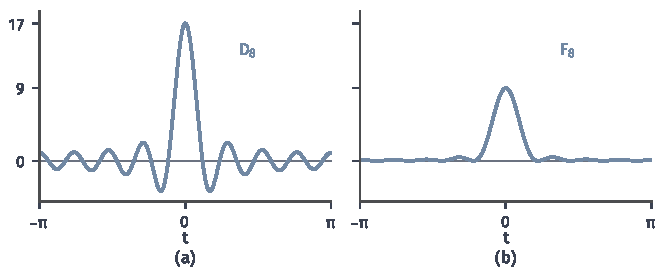
\includegraphics[width=112mm]{figures/04-spaces-measures-and-geometry/03-function-spaces/matplotlib/fourier-kernels/figure.pdf}
  \caption{$N=8$时的两个核，纵轴相同。(a)Dirichlet核$D_8$在$t=0$处高$17$，两侧正负交替。(b)Fejér核$F_8$在$t=0$处高$9$，处处非负，远离原点时几乎为零。}
  \label{fig:fourier-kernels}
\end{BookInlineFigure}

$F_N$有三条性质，恰好是把它当作“集中于原点的权”所需要的，图~\ref{fig:fourier-kernels}(b)可以对照：
\begin{itemize}
\item $F_N\geq0$，这从式~\eqref{eq:fourier-fejer-closed}直接读出；
\item $\frac1{2\pi}\int_{-\pi}^{\pi}F_N=1$，因为每个$D_n$只有常数项$1$对积分有贡献；
\item 对$0<\delta\leq\lvert t\rvert\leq\pi$，$F_N(t)\leq\dfrac1{(N+1)\sin^2(\delta/2)}$，所以质量随$N$增大集中到原点附近。
\end{itemize}

\begin{lemma}[Fejér平均的收敛]
\label{lem:fourier-fejer}
若$f$是连续的周期函数，则$\sigma_Nf$一致收敛到$f$。若$f\in L^2(\mathbb T)$，则$\lVert\sigma_Nf-f\rVert_2\to0$。
\end{lemma}

\begin{proof}
由$F_N$的积分为$1$，把$f(x)$写进积分，得到
\[
\sigma_Nf(x)-f(x)=\frac1{2\pi}\int_{-\pi}^{\pi}\bigl(f(x-t)-f(x)\bigr)F_N(t)\,\mathrm dt.
\]

先看连续的$f$。它在紧区间上一致连续，记
\[
\omega(\delta)=\sup_{\lvert t\rvert<\delta}\sup_x\lvert f(x-t)-f(x)\rvert,
\]
则$\delta\to0$时$\omega(\delta)\to0$。把积分分成$\lvert t\rvert<\delta$与$\delta\leq\lvert t\rvert\leq\pi$两部分。前一部分用$\omega(\delta)$控制差、用积分为$1$控制权；后一部分把差的绝对值放大为$2\lVert f\rVert_\infty$，再用$F_N$的第三条性质。于是
\[
\lvert\sigma_Nf(x)-f(x)\rvert\leq\omega(\delta)+\frac{2\lVert f\rVert_\infty}{(N+1)\sin^2(\delta/2)}.
\]
右边与$x$无关。先取$\delta$使第一项小，再令$N$充分大使第二项小，即得一致收敛。

再看$f\in L^2(\mathbb T)$。由前两条性质，$\frac1{2\pi}F_N(t)\,\mathrm dt$是一个周期上的概率测度。对它用Cauchy--Schwarz不等式，得到
\[
\lvert\sigma_Nf(x)-f(x)\rvert^2\leq\frac1{2\pi}\int_{-\pi}^{\pi}\lvert f(x-t)-f(x)\rvert^2F_N(t)\,\mathrm dt.
\]
对$x$按归一化测度积分，并用Tonelli定理交换次序。记平移$(\tau_tf)(x)=f(x-t)$，于是
\[
\lVert\sigma_Nf-f\rVert_2^2\leq\frac1{2\pi}\int_{-\pi}^{\pi}\lVert\tau_tf-f\rVert_2^2\,F_N(t)\,\mathrm dt.
\]
同样分成$\lvert t\rvert<\delta$与其余部分，并用$\lVert\tau_tf-f\rVert_2\leq2\lVert f\rVert_2$。这样只需再说明$t\to0$时$\lVert\tau_tf-f\rVert_2\to0$。

这一平移连续性分三步得到。第~\ref{chap:smoothing-weak-derivatives}章证明了$\mathbb R$上的可积函数$F$满足$\int\lvert F(x-h)-F(x)\rvert\,\mathrm dx\to0$。对周期函数$f$与$\lvert h\rvert\leq\pi$，取$F=f\mathbf 1_{[-2\pi,2\pi]}$，在$x\in[-\pi,\pi]$上$F(x-h)=f(x-h)$，所以周期情形的$L^1$平移连续性成立。

若还有$\lvert f\rvert\leq n$，则
\[
\lvert\tau_hf-f\rvert^2\leq2n\,\lvert\tau_hf-f\rvert,
\]
所以有界函数的$L^2$平移连续性成立。

对一般的$f\in L^2(\mathbb T)$，取$f_n=f\mathbf 1_{\{\lvert f\rvert\leq n\}}$。由控制收敛定理，$\lVert f-f_n\rVert_2\to0$。平移不改变周期函数的范数，所以
\[
\lVert\tau_hf-f\rVert_2\leq2\lVert f-f_n\rVert_2+\lVert\tau_hf_n-f_n\rVert_2.
\]
先取$n$使第一项小，再令$h\to0$，第二项趋于零。
\end{proof}

\paragraph{完备性与Parseval关系}

$\sigma_Nf$完全由Fourier系数决定，这正是证明完备性所需要的。

\begin{theorem}[$L^2$中的Fourier展开]
\label{thm:fourier-series-l2}
$\{e_k\}_{k\in\mathbb Z}$是$L^2(\mathbb T)$的完备标准正交系。因此对每个$f\in L^2(\mathbb T)$，$\lVert S_Nf-f\rVert_2\to0$，并且
\begin{equation}
\begin{gathered}
\frac1{2\pi}\int_{-\pi}^{\pi}\lvert f(x)\rvert^2\,\mathrm dx=\sum_{k\in\mathbb Z}\lvert\widehat f(k)\rvert^2 ,\\
\langle f,g\rangle=\sum_{k\in\mathbb Z}\overline{\widehat f(k)}\,\widehat g(k) .
\end{gathered}
\label{eq:fourier-series-parseval}
\end{equation}
\end{theorem}

\begin{proof}
设$f\in L^2(\mathbb T)$与每个$e_k$正交，即全部$\widehat f(k)=0$。则每个$S_nf=0$，从而$\sigma_Nf=0$。由引理~\ref{lem:fourier-fejer}，$\sigma_Nf\to f$于$L^2$，所以$f=0$。完备标准正交系的范数收敛展开、Parseval等式及内积公式，由第~\ref{chap:function-inner-product-spaces}章的正交展开定理给出。
\end{proof}

式~\eqref{eq:fourier-series-parseval}就是无限维的勾股定理：一个周期上的平均能量等于各坐标模平方之和，本章称为Parseval关系。截断误差也由它读出，投影与残差正交，所以
\begin{equation}
\lVert f-S_Nf\rVert_2^2=\sum_{\lvert k\rvert>N}\lvert\widehat f(k)\rvert^2 .
\label{eq:fourier-series-truncation}
\end{equation}

结合第~\ref{chap:function-inner-product-spaces}章的结论，$f\mapsto(\widehat f(k))_{k\in\mathbb Z}$是$L^2(\mathbb T)$到$\ell^2(\mathbb Z)$的保持内积的双射。在$L^2$的意义下，“函数是一列坐标”这句话是严格成立的。

用方波核对一下。左边的平均能量为$1$，右边只有奇数$k$有贡献，每个模平方为$4/(\pi^2k^2)$，$\pm k$各一项，所以
\[
1=2\sum_{j\geq0}\frac{4}{\pi^2(2j+1)^2}.
\]
整理后得到一个级数的值：
\[
\sum_{j\geq0}\frac1{(2j+1)^2}=\frac{\pi^2}8 .
\]

截断误差也可以逐项算出。前几项的平方和分别是
\[
\frac8{\pi^2}\approx0.8106,\qquad
\frac8{\pi^2}\Bigl(1+\frac19\Bigr)\approx0.9006,\qquad
\frac8{\pi^2}\Bigl(1+\frac19+\frac1{25}\Bigr)\approx0.9331.
\]
由式~\eqref{eq:fourier-series-truncation}，$\lVert f-S_Nf\rVert_2^2$在$N=1,3,5$时分别约为$0.1894$、$0.0994$、$0.0669$。每增加一个坐标，误差平方恰好减少该坐标的模平方，已经算好的系数不必修改，这是正交基的好处。系数的衰减怎样决定误差的速度，留到第~\ref{chap:function-approximation}章研究。

\paragraph{实形式与一般周期}

实值函数也常用正弦与余弦展开。若$f$为实值，对式~\eqref{eq:fourier-coefficient}取共轭得到$\widehat f(-k)=\overline{\widehat f(k)}$。把$\pm k$两项配对，就得到实形式：
\[
f\sim\frac{a_0}2+\sum_{k\geq1}\bigl(a_k\cos kx+b_k\sin kx\bigr),
\]
其中
\[
a_k=\frac1\pi\int_{-\pi}^{\pi}f(x)\cos kx\,\mathrm dx,\qquad
b_k=\frac1\pi\int_{-\pi}^{\pi}f(x)\sin kx\,\mathrm dx.
\]
两套系数的关系是
\[
\widehat f(0)=\frac{a_0}2,\qquad\widehat f(k)=\frac{a_k-\mathrm ib_k}2\quad(k\geq1).
\]
相应地，Parseval关系写成
\[
\frac1{2\pi}\int_{-\pi}^{\pi}\lvert f\rvert^2=\frac{a_0^2}4+\frac12\sum_{k\geq1}(a_k^2+b_k^2).
\]

两种写法表示同一个展开，实形式中的$1/\pi$与$1/2$都来自配对。方波的实系数是$a_k=0$，奇数$k$时$b_k=4/(\pi k)$，与例~\ref{ex:fourier-square-wave}一致。这相当于把同一组坐标换成实的基$1,\sqrt2\cos kx,\sqrt2\sin kx$来写，只是常数放的位置不同。

若周期是$T$而不是$2\pi$，令$x=2\pi t/T$即可化归本节情形。这时系数为
\begin{equation}
c_k=\frac1T\int_0^Tf(t)\,e^{-2\pi\mathrm ikt/T}\,\mathrm dt ,
\label{eq:fourier-period-T}
\end{equation}
第$k$个基函数的频率是单位长度内$k/T$圈。周期越长，相邻频率越靠近，这一点在下一节开头会用到。

\paragraph{系数描述的是等价类}

类比还有一个需要注意的地方。Fourier系数是积分，改变$f$在一个零测集上的值不改变任何坐标。所以坐标记录的不是一张逐点的取值表，而是$L^2(\mathbb T)$中的一个等价类。定理~\ref{thm:fourier-series-l2}中的展开是范数意义下的等式，不是逐点等式。

例~\ref{ex:fourier-square-wave}中没有规定方波在$0$和$\pm\pi$处的取值，原因就在这里：无论在这些点赋什么值，算出来的系数都一样，$\pi^2/8$这个结果也一样。要讨论$S_Nf$在某一点的值，必须另外加条件，这是下一小节的内容。

\subsection{点态收敛}
\label{sec:fourier-series-pointwise}

$L^2$收敛控制的是一个周期上的平均平方误差，它不告诉我们部分和在某个给定点处是否收敛。连续性也不够：du Bois-Reymond构造过连续周期函数，其Fourier级数在某一点发散，构造较长，读者可查阅Fourier分析的教材。所以逐点结论必须对$f$加上比连续更强的局部条件，本小节使用分段$C^1$条件。

\paragraph{Riemann--Lebesgue引理}

逐点收敛的证明最终要说明一个高频振荡积分趋于零。直观上，$g(t)e^{-\mathrm i\lambda t}$在长度为$\pi/\lambda$的小段上一正一负，而$g$在这么短的距离上几乎不变，正负两部分几乎抵消。这件事对任何可积函数都成立。

\begin{lemma}[Riemann--Lebesgue引理]
\label{lem:fourier-riemann-lebesgue}
若$g\in L^1(\mathbb R)$，则$\lvert\lambda\rvert\to\infty$时
\begin{equation}
\int_{\mathbb R}g(t)e^{-\mathrm i\lambda t}\,\mathrm dt\to0 .
\label{eq:fourier-riemann-lebesgue}
\end{equation}
特别地，$\int g(t)\sin(\lambda t)\,\mathrm dt\to0$；对$f\in L^1(\mathbb T)$，$\lvert k\rvert\to\infty$时$\widehat f(k)\to0$。
\end{lemma}

\begin{proof}
把式~\eqref{eq:fourier-riemann-lebesgue}左边的积分记为$I(\lambda)$，$\lambda\neq0$。作换元$t\mapsto t+\pi/\lambda$，并用$e^{-\mathrm i\pi}=-1$，得到
\[
I(\lambda)=-\int_{\mathbb R}g(t+\pi/\lambda)\,e^{-\mathrm i\lambda t}\,\mathrm dt.
\]
把它与原式相加再取模，得到
\[
2\lvert I(\lambda)\rvert\leq\int_{\mathbb R}\lvert g(t)-g(t+\pi/\lambda)\rvert\,\mathrm dt.
\]
由第~\ref{chap:smoothing-weak-derivatives}章的平移积分连续性，右边在$\lvert\lambda\rvert\to\infty$时趋于零。对$\lambda$取实部虚部即得正弦情形。周期情形把$f$在一个周期外置零，再取$\lambda=k$。
\end{proof}

对$L^2$函数，坐标趋于零可以由Bessel不等式读出，因为平方可和的序列必趋于零。引理的新内容在于它只要求可积，而$L^1(\mathbb T)$函数的坐标不必平方可和。它也不给出趋于零的速度：方波的系数按$1/\lvert k\rvert$衰减，后面会看到更光滑的函数衰减得更快。

\paragraph{分段$C^1$函数的Dirichlet定理}

称周期函数$f$为分段$C^1$，是指在一个周期$[-\pi,\pi]$中有有限个分点，使$f$在每个开子区间上连续可微，并且$f$与$f'$在每个子区间端点处有单侧极限。于是在每一点$x$都存在单侧极限$f(x+)$与$f(x-)$，它们在连续点相等，在跳跃点不等。方波是最典型的例子。

\begin{theorem}[Dirichlet定理]
\label{thm:fourier-dirichlet}
设$f$是分段$C^1$的$2\pi$周期函数，则对每个$x\in\mathbb R$，
\begin{equation}
\lim_{N\to\infty}S_Nf(x)=\frac{f(x+)+f(x-)}2 .
\label{eq:fourier-dirichlet-limit}
\end{equation}
特别地，在$f$的连续点，$S_Nf(x)\to f(x)$。
\end{theorem}

\begin{proof}
$D_N$是偶函数，所以式~\eqref{eq:fourier-dirichlet-integral}可以按$t>0$与$t<0$合并为
\[
S_Nf(x)=\frac1{2\pi}\int_0^{\pi}\bigl[f(x+t)+f(x-t)\bigr]D_N(t)\,\mathrm dt.
\]
又由$D_N$的积分得$\frac1{2\pi}\int_0^{\pi}D_N=\frac12$，因此可以把左右极限的平均写进同一个积分。记
\[
h(t)=f(x+t)-f(x+)+f(x-t)-f(x-),
\]
并利用式~\eqref{eq:fourier-dirichlet-closed}，得到
\[
S_Nf(x)-\frac{f(x+)+f(x-)}2=\frac1{2\pi}\int_0^{\pi}\frac{h(t)}{\sin(t/2)}\sin\bigl((N+\tfrac12)t\bigr)\,\mathrm dt.
\]
只需说明$g(t)=h(t)/\sin(t/2)$在$(0,\pi)$上可积，然后对$g\mathbf 1_{(0,\pi)}$用引理~\ref{lem:fourier-riemann-lebesgue}。

取$t_0>0$，小于$x$到两侧最近分点的距离。在$(x,x+t_0)$上$f$连续可微，$f'$有单侧极限，所以$\lvert f'\rvert\leq C$。对$0<s<t<t_0$用中值定理，得到$\lvert f(x+t)-f(x+s)\rvert\leq C(t-s)$。令$s\to0^+$，得到
\[
\lvert f(x+t)-f(x+)\rvert\leq Ct.
\]
左侧同理。又$0\leq t\leq\pi$时$\sin(t/2)\geq t/\pi$，所以$g$在$(0,t_0)$上有界。在$[t_0,\pi]$上，$\sin(t/2)\geq\sin(t_0/2)>0$，而$f$有界，$g$也有界。因此$g$可积，引理给出右边趋于零。
\end{proof}

\paragraph{连续点、跳跃点与等价类}

定理把每一点分成两类，用方波可以逐一核对。取连续点$x=\pi/2$，这时$\sin(k\pi/2)$对$k=1,3,5,\ldots$依次为$1,-1,1,\ldots$，所以
\[
S_Nf\Bigl(\frac\pi2\Bigr)=\frac4\pi\Bigl(1-\frac13+\frac15-\cdots\Bigr).
\]
$N=1,3,5,7$时的值依次约为$1.273$、$0.849$、$1.104$、$0.922$，在$f(\pi/2)=1$的两侧摆动着收敛。

再取跳跃点$x=0$。每个$\sin(k\cdot0)=0$，所以$S_Nf(0)=0$对一切$N$成立，这正是左右极限的平均$(1+(-1))/2$。无论在$0$处给方波赋什么值，极限都是$0$：单点赋值既不进入系数，也不进入单侧极限。

与$L^2$展开相比，这里多用了$x$两侧的单侧Lipschitz估计，它来自分段$C^1$假设，使$g$在$t=0$附近可积；Riemann--Lebesgue引理本身只需要可积性。证明还显示了收敛的局部性：$g$只在$x$附近需要特别的估计，远离$x$处只用了有界性。$L^2$收敛不能代替这里的局部条件，因为它允许在零测集上任意修改函数，而逐点问题恰恰关心单个点。

\subsection{一致收敛}
\label{sec:fourier-series-uniform}

点态收敛允许不同点以不同速度收敛，一致收敛则要求整个周期上的最大误差趋于零。一个简单的充分条件是坐标绝对可和，而坐标衰减的速度由函数的光滑性控制。

\paragraph{分部积分与系数衰减}

对连续可微的周期函数，分部积分把求导转到坐标上。在$\widehat{f'}(k)$的定义中分部积分，得到
\[
\widehat{f'}(k)=\frac1{2\pi}\Bigl[f(x)e^{-\mathrm ikx}\Bigr]_{-\pi}^{\pi}+\frac{\mathrm ik}{2\pi}\int_{-\pi}^{\pi}f(x)e^{-\mathrm ikx}\,\mathrm dx.
\]
$f$与$e^{-\mathrm ikx}$都以$2\pi$为周期，边界项为零，所以
\begin{equation}
\widehat{f'}(k)=\mathrm ik\,\widehat f(k).
\label{eq:fourier-series-derivative}
\end{equation}
求导在这组坐标下是对角矩阵$\operatorname{diag}(\mathrm ik)$。这一步依赖周期性：若$f(\pi)\neq f(-\pi)$，边界项不为零。

\begin{theorem}[$C^2$函数的一致收敛]
\label{thm:fourier-uniform}
设$f$是二次连续可微的$2\pi$周期函数。则对$k\neq0$有
\begin{equation}
\lvert\widehat f(k)\rvert\leq\frac{\lVert f''\rVert_\infty}{k^2},
\label{eq:fourier-c2-coefficient}
\end{equation}
$\sum_k\lvert\widehat f(k)\rvert<\infty$，并且$S_Nf$一致收敛到$f$，
\begin{equation}
\sup_x\lvert f(x)-S_Nf(x)\rvert\leq\frac{2\lVert f''\rVert_\infty}{N},\qquad N\geq1 .
\label{eq:fourier-c2-uniform-error}
\end{equation}
\end{theorem}

\begin{proof}
用式~\eqref{eq:fourier-series-derivative}两次，得到$\widehat{f''}(k)=-k^2\widehat f(k)$。而$\widehat{f''}(k)$的模不超过$\lVert f''\rVert_1\leq\lVert f''\rVert_\infty$，这给出系数估计。

由$\sum_{k\neq0}k^{-2}<\infty$，Weierstrass判别法说明$S_Nf$一致收敛到某个连续函数$h$。一致收敛蕴含$L^2$收敛，而定理~\ref{thm:fourier-series-l2}说明$S_Nf\to f$于$L^2$，所以$h=f$几乎处处。两个连续函数若在某点不等，就在该点的一个邻域内不等，邻域的测度为正，所以$h=f$处处成立。

误差估计来自尾部求和。对每个$x$，误差不超过被舍弃坐标的模之和：
\[
\lvert f(x)-S_Nf(x)\rvert\leq\sum_{\lvert k\rvert>N}\lvert\widehat f(k)\rvert.
\]
由式~\eqref{eq:fourier-c2-coefficient}，只需估计$k^{-2}$的尾部和：
\[
\sum_{\lvert k\rvert>N}\frac1{k^2}=2\sum_{k>N}\frac1{k^2}\leq2\int_N^\infty\frac{\mathrm dt}{t^2}=\frac2N.
\]
乘上$\lVert f''\rVert_\infty$，就是式~\eqref{eq:fourier-c2-uniform-error}。
\end{proof}

$C^2$只是一个方便的充分条件，连续可微就已足够。由式~\eqref{eq:fourier-series-derivative}与Cauchy--Schwarz不等式，
\[
\sum_{k\neq0}\lvert\widehat f(k)\rvert=\sum_{k\neq0}\frac{\lvert\widehat{f'}(k)\rvert}{\lvert k\rvert}
\leq\lVert f'\rVert_2\Bigl(\sum_{k\neq0}\frac1{k^2}\Bigr)^{1/2},
\]
这里用到$f'$的Parseval关系。

不必处处可导。周期延拓的$\lvert x\rvert$（三角波）在$0$与$\pm\pi$处有尖点，分部积分得到它的系数：
\[
\widehat f(0)=\frac\pi2,\qquad
\widehat f(k)=\frac{(-1)^k-1}{\pi k^2}\quad(k\neq0).
\]
奇数$k$时$\widehat f(k)=-2/(\pi k^2)$，偶数$k\neq0$时为零，绝对可和，所以部分和一致收敛，极限与$f$处处相等的论证同上。

在$x=0$处取值，右边是$\pi/2$减去正数项，得到
\[
0=\frac\pi2-\frac4\pi\sum_{j\geq0}\frac1{(2j+1)^2},
\]
这与方波的Parseval关系给出的$\pi^2/8$一致。逐项算，$N=1,3,5,9$时$S_Nf(0)$依次约为$0.298$、$0.156$、$0.105$、$0.064$，趋于$f(0)=0$。

比较两个例子。方波有跳跃，系数按$1/\lvert k\rvert$衰减，不绝对可和；三角波连续，只有尖点，系数按$1/k^2$衰减，绝对可和。函数越光滑，高频坐标越小。

\paragraph{三种误差的比较}

三种收敛方式衡量的是不同的误差。一致误差$\sup_x\lvert f-S_Nf\rvert$控制每一点，因而控制逐点误差。由$\lVert\cdot\rVert_2\leq\sup\lvert\cdot\rvert$，它也控制$L^2$误差。反过来，$L^2$误差小只说明误差大的地方测度小，逐点收敛也可以在不同点有不同速度。

跳跃函数不能获得一致收敛。部分和$S_Nf$是三角多项式，处处连续；一致收敛的连续函数列的极限连续，可参考\BookChapterRef{chap:limits-continuity}{卷一第5章“极限与连续”}。方波在$0$处跳跃，所以$S_Nf$不可能一致收敛到任何与方波几乎处处相等的函数。

具体的情形可以算出来。取$N=2n-1$，对$S_Nf$求导，用几何级数求和得
\[
(S_Nf)'(x)=\frac4\pi\sum_{j=1}^n\cos\bigl((2j-1)x\bigr)=\frac2\pi\cdot\frac{\sin 2nx}{\sin x}.
\]
所以在$x>0$一侧，第一个峰出现在$x=\pi/(2n)$。把这一点代入$S_Nf$，并记$x_j=(2j-1)\pi/(2n)$，有$\frac1{2j-1}=\frac{\pi}{2n\,x_j}$，于是
\[
S_Nf\Bigl(\frac\pi{2n}\Bigr)=\frac2\pi\sum_{j=1}^n\frac{\sin x_j}{x_j}\cdot\frac\pi n.
\]
右边是$\sin u/u$在$[0,\pi]$上步长$\pi/n$的中点Riemann和，所以$n\to\infty$时
\[
S_Nf\Bigl(\frac\pi{2n}\Bigr)\to\frac2\pi\int_0^\pi\frac{\sin u}{u}\,\mathrm du\approx1.179.
\]
这就是\term{Gibbs现象}（Gibbs phenomenon）：跳跃附近的部分和总要越过跳跃高度，超出约$0.179$，即跳跃幅度$2$的约$9\%$，而峰的位置随$N$增大向跳跃点收缩。$N=9,25,81$时峰值依次约为$1.182$、$1.180$、$1.179$。

\begin{BookInlineFigure}
  \centering
  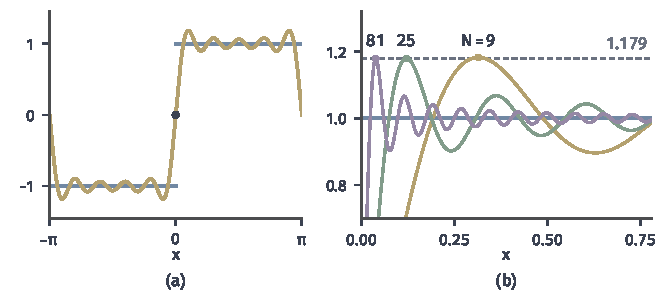
\includegraphics[width=112mm]{figures/04-spaces-measures-and-geometry/03-function-spaces/matplotlib/fourier-gibbs/figure.pdf}
  \caption{方波的Gibbs现象。蓝色为方波。(a)$N=9$的部分和（黄色），在跳跃点$0$处取值$0$（黑点）。(b)$x>0$一侧的放大图，黄、绿、紫分别为$N=9,25,81$，圆点是各自的第一个峰，都接近虚线$1.179$，峰随$N$增大靠近跳跃点。}
  \label{fig:fourier-gibbs}
\end{BookInlineFigure}

图~\ref{fig:fourier-gibbs}(b)说明这与定理~\ref{thm:fourier-dirichlet}并不矛盾。固定一个$x>0$，峰迟早越过它，之后$S_Nf(x)$趋于$1$；只是越靠近跳跃点，收敛越晚，所以最大误差始终不小。三种误差在方波上的表现是：$L^2$误差趋于零，每个固定点的误差趋于零，而一致误差不趋于零。

\section{\texorpdfstring{$L^1$}{L1}中的Fourier变换}
\label{sec:fourier-l1}

非周期函数不能在一个周期上读坐标，但上一节末尾已经提示了办法：周期$T$越长，频率$k/T$越密。对定义在整个$\mathbb R^d$上的函数，频率应当取遍$\mathbb R^d$，对整数$k$的求和换成对频率$\xi$的积分。向量的下标从整数连成了整个空间，这是类比的又一次推广，也是它开始变得不严格的地方。

本节先在绝对可积函数上建立变换本身，再单独回答怎样从频率函数还原原函数。

\subsection{Fourier变换的基本性质}
\label{sec:fourier-l1-properties}

\paragraph{定义与归一化}

先用一个周期很长的函数看看下标是怎样连起来的。设$f$是实轴上的可积函数，支撑在$[-T/2,T/2]$内，把它按$T$周期延拓。由式~\eqref{eq:fourier-period-T}，它的系数$c_k$乘$T$之后是
\[
Tc_k=\int_{-T/2}^{T/2}f(x)\,e^{-2\pi\mathrm i(k/T)x}\,\mathrm dx .
\]
只要$T$足够大，右边的积分就不再依赖$T$，它只依赖频率$\xi=k/T$，是同一个函数$\xi\mapsto\int f(x)e^{-2\pi\mathrm ix\xi}\,\mathrm dx$在格点$k/T$上的取值。

取方框$B=\mathbf 1_{[-1/2,1/2]}$算一个具体的值。取$T=2$、$k=1$，频率是$\xi=1/2$，于是
\[
2c_1=\int_{-1/2}^{1/2}e^{-\mathrm i\pi x}\,\mathrm dx=\frac{\sin(\pi/2)}{\pi/2}=\frac2\pi\approx0.637.
\]
图~\ref{fig:fourier-series-to-transform}画出$T=2,4,8$时的全部$Tc_k$：它们落在同一条曲线上，$T$每增大一倍，取样点就密一倍。

\begin{BookInlineFigure}
  \centering
  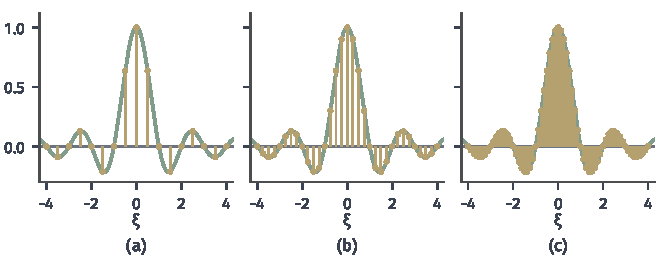
\includegraphics[width=112mm]{figures/04-spaces-measures-and-geometry/03-function-spaces/matplotlib/fourier-series-to-transform/figure.pdf}
  \caption{周期增大时系数连成曲线。方框$B$按周期$T$延拓，黄色竖线为$Tc_k$，位于频率$k/T$处。(a)$T=2$。(b)$T=4$。(c)$T=8$。绿色曲线是极限对象$\sin(\pi\xi)/(\pi\xi)$，三幅图中相同。}
  \label{fig:fourier-series-to-transform}
\end{BookInlineFigure}

展开式也随之变形。把$c_k$代入周期$T$的Fourier级数，得到
\[
f(x)=\sum_{k\in\mathbb Z}\Bigl(\int f(y)e^{-2\pi\mathrm i(k/T)y}\,\mathrm dy\Bigr)\,e^{2\pi\mathrm i(k/T)x}\cdot\frac1T .
\]
右边是一个频率步长为$1/T$的Riemann和。$T\to\infty$时，它的形式极限是对$\xi$的积分。这只是启发，下面的定义和证明不依赖这个极限过程。

对$x,\xi\in\mathbb R^d$，记$x\cdot\xi=\sum_ix_i\xi_i$。函数$x\mapsto e^{2\pi\mathrm ix\cdot\xi}$沿方向$\xi/\lvert\xi\rvert$每前进$1/\lvert\xi\rvert$就转一圈，所以$\lvert\xi\rvert$是单位长度内的圈数，这样的函数称为平面波。

\begin{definition}[Fourier变换]
\label{def:fourier-transform-l1}
对$f\in L^1(\mathbb R^d)$，定义它的\term{Fourier变换}（Fourier transform）为
\begin{equation}
\widehat f(\xi)=\int_{\mathbb R^d}f(x)e^{-2\pi\mathrm ix\cdot\xi}\,\mathrm dx ,\qquad\xi\in\mathbb R^d .
\label{eq:fourier-transform-l1}
\end{equation}
\end{definition}

由于指数因子的模恒为$1$，可积性保证积分对每个$\xi$都存在，并且改变$f$在零测集上的值不影响结果。所以$\widehat f$是一个在每个频率处都有确定值的函数，这一点到$L^2$情形会改变。

类比在这里要打一个折扣。式~\eqref{eq:fourier-transform-l1}形式上是“与平面波作内积”，但平面波的模恒为$1$，在$\mathbb R^d$上既不可积也不平方可积，它们不是$L^2(\mathbb R^d)$中的元素，更谈不上构成正交基。可以把$\widehat f(\xi)$想成下标为$\xi$的坐标，但一切结论都要直接证明，不能照搬Hilbert空间的展开定理。

指数中的$2\pi$是一种约定。另一种常见写法用角频率$\omega=2\pi\xi$，把指数换成$e^{-\mathrm ix\cdot\omega}$，所得函数记为$F(\omega)$，两者只差自变量的伸缩，$F(\omega)=\widehat f(\omega/2\pi)$。约定不改变任何结论，只改变反演与能量公式中的常数；本章始终采用定义中的写法，第~\ref{sec:fourier-l2}节末尾给出常数的对照。

\paragraph{有界性、连续性与高频衰减}

和周期情形一样，可积性已经足以给出变换的几条基本性质。

\begin{theorem}[$L^1$上Fourier变换的基本性质]
\label{thm:fourier-l1-properties}
设$f,g\in L^1(\mathbb R^d)$，$a,b\in\mathbb C$。则
\begin{enumerate}
\item $\widehat{af+bg}=a\widehat f+b\widehat g$，且$\lVert\widehat f\rVert_\infty\leq\lVert f\rVert_1$；
\item $\widehat f$在$\mathbb R^d$上连续；
\item $\lvert\xi\rvert\to\infty$时$\widehat f(\xi)\to0$。
\end{enumerate}
\end{theorem}

\begin{proof}
线性来自积分的线性。有界性来自
\[
\lvert\widehat f(\xi)\rvert\leq\int_{\mathbb R^d}\lvert f(x)e^{-2\pi\mathrm ix\cdot\xi}\rvert\,\mathrm dx=\lVert f\rVert_1.
\]

连续性：若$\xi_n\to\xi$，被积函数逐点收敛到$f(x)e^{-2\pi\mathrm ix\cdot\xi}$，并被可积函数$\lvert f\rvert$控制。由控制收敛定理，$\widehat f(\xi_n)\to\widehat f(\xi)$。

高频衰减与引理~\ref{lem:fourier-riemann-lebesgue}的证明相同。对$\xi\neq0$取
\[
h=\frac{\xi}{2\lvert\xi\rvert^2},
\]
则$e^{-2\pi\mathrm ih\cdot\xi}=e^{-\pi\mathrm i}=-1$。作换元$x\mapsto x+h$，得到
\[
\widehat f(\xi)=-\int_{\mathbb R^d}f(x+h)\,e^{-2\pi\mathrm ix\cdot\xi}\,\mathrm dx.
\]
与原式相加再取模，得到
\[
2\lvert\widehat f(\xi)\rvert\leq\int_{\mathbb R^d}\lvert f(x)-f(x+h)\rvert\,\mathrm dx.
\]
$\lvert\xi\rvert\to\infty$时$\lvert h\rvert=1/(2\lvert\xi\rvert)\to0$，由第~\ref{chap:smoothing-weak-derivatives}章的平移积分连续性，右边趋于零。
\end{proof}

于是$f\mapsto\widehat f$把$L^1(\mathbb R^d)$线性地映到在无穷远处趋于零的有界连续函数中，而且不增加相应的范数。第3条也称为Riemann--Lebesgue引理。它不给出衰减速度，速度与$f$的光滑性有关，第~\ref{sec:fourier-operations}节的微分规则会给出具体联系。

\paragraph{三个例子}

先算两个一维例子。第一个是中心方框$B=\mathbf 1_{[-1/2,1/2]}$。直接积分，对$\xi\neq0$有
\begin{equation}
\widehat B(\xi)=\int_{-1/2}^{1/2}e^{-2\pi\mathrm ix\xi}\,\mathrm dx=\frac{\sin(\pi\xi)}{\pi\xi},
\label{eq:fourier-box}
\end{equation}
并且$\widehat B(0)=1$。零点在非零整数处，例如$\widehat B(1/2)=2/\pi$，与上面周期化时算出的$2c_1$相同。

$\widehat B$连续，在无穷远处趋于零，但只按$1/\lvert\xi\rvert$衰减，在$\mathbb R$上不绝对可积。事实上，在每个区间$[n,n+1]$（$n\geq1$）上，分母不超过$\pi(n+1)$，而$\lvert\sin\pi\xi\rvert$在长度为$1$的区间上的积分是$2/\pi$，所以
\[
\int_n^{n+1}\frac{\lvert\sin\pi\xi\rvert}{\pi\lvert\xi\rvert}\,\mathrm d\xi\geq\frac{2}{\pi^2(n+1)}.
\]
对$n$求和，调和级数发散。

第二个例子是双边指数$f(x)=e^{-\lvert x\rvert}$。把积分分成$x>0$与$x<0$两段，第二段作换元$x\mapsto-x$，得到
\[
\widehat f(\xi)=\int_0^\infty e^{-x(1+2\pi\mathrm i\xi)}\,\mathrm dx+\int_0^\infty e^{-x(1-2\pi\mathrm i\xi)}\,\mathrm dx.
\]
每段都是指数积分，所以
\[
\widehat f(\xi)=\frac1{1+2\pi\mathrm i\xi}+\frac1{1-2\pi\mathrm i\xi}.
\]
通分，得到
\begin{equation}
\widehat f(\xi)=\frac{2}{1+4\pi^2\xi^2}.
\label{eq:fourier-double-exponential}
\end{equation}
它按$1/\xi^2$衰减，是可积的。检验一下：$\widehat f(0)=2$，正是$\int e^{-\lvert x\rvert}\,\mathrm dx$的值。

第三个例子是Gauss函数$G(x)=e^{-\pi\lvert x\rvert^2}$，它的变换就是它自己：$\widehat G=G$。先看$d=1$。由极坐标（二重积分的换元可参考\BookChapterRef{chap:region-integrals}{卷二第24章“区域积分”}），
\[
\Bigl(\int_{\mathbb R}e^{-\pi x^2}\,\mathrm dx\Bigr)^2=\int_0^{2\pi}\int_0^\infty e^{-\pi r^2}r\,\mathrm dr\,\mathrm d\theta=1,
\]
所以$\int e^{-\pi x^2}\,\mathrm dx=1$。

再令$\varphi(\xi)=\widehat G(\xi)$。由于$\lvert x\rvert e^{-\pi x^2}$可积，可以在积分号下对$\xi$求导（第~\ref{chap:integration}章的含参积分求导条件）。注意$(e^{-\pi x^2})'=-2\pi xe^{-\pi x^2}$，于是
\[
\varphi'(\xi)=\int(-2\pi\mathrm ix)e^{-\pi x^2}e^{-2\pi\mathrm ix\xi}\,\mathrm dx
=\mathrm i\int\bigl(e^{-\pi x^2}\bigr)'e^{-2\pi\mathrm ix\xi}\,\mathrm dx.
\]
分部积分，边界项因$e^{-\pi x^2}\to0$而消失，得到
\[
\varphi'(\xi)=\mathrm i\cdot2\pi\mathrm i\xi\,\varphi(\xi)=-2\pi\xi\,\varphi(\xi).
\]
这个常微分方程配上初值$\varphi(0)=\int e^{-\pi x^2}\,\mathrm dx=1$，解得$\varphi(\xi)=e^{-\pi\xi^2}$。$d$维时，$G(x)e^{-2\pi\mathrm ix\cdot\xi}$是各坐标函数的乘积，由Fubini定理逐坐标积分即得$\widehat G=G$。

图~\ref{fig:fourier-three-pairs}把三对函数放在一起。从左到右，原函数越来越光滑：方框有跳跃，双边指数只有一个尖点，Gauss函数无穷次可导。下方的变换衰减也越来越快，依次是$1/\lvert\xi\rvert$、$1/\xi^2$与快于任何多项式。这是周期情形“越光滑，高频坐标越小”的连续版本。

\begin{BookInlineFigure}
  \centering
  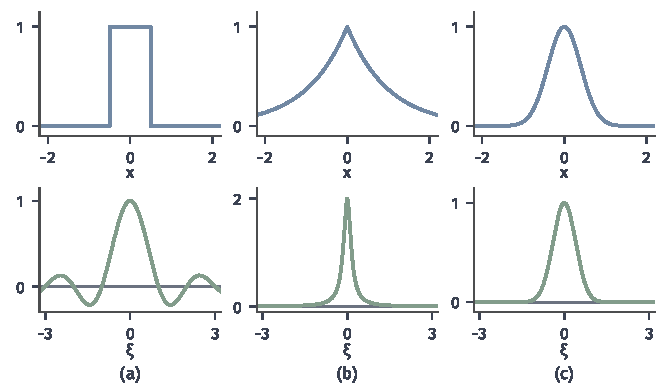
\includegraphics[width=112mm]{figures/04-spaces-measures-and-geometry/03-function-spaces/matplotlib/fourier-three-pairs/figure.pdf}
  \caption{三个Fourier变换对。上排蓝色为原函数，下排绿色为对应的变换。(a)方框$B$与$\sin(\pi\xi)/(\pi\xi)$。(b)双边指数$e^{-\lvert x\rvert}$与$2/(1+4\pi^2\xi^2)$，注意纵轴到$2$。(c)Gauss函数$e^{-\pi x^2}$与它自身。}
  \label{fig:fourier-three-pairs}
\end{BookInlineFigure}

\paragraph{平移、缩放与变换的定义域}

原函数作平移或缩放之后，仍属于$L^1(\mathbb R^d)$，它的变换仍是$\mathbb R^d$上全体频率的函数，变化的只是取值。例如加宽一倍的方框$B(x/2)=\mathbf 1_{[-1,1]}$，直接积分得到
\[
\widehat{B(\cdot/2)}(\xi)=\frac{\sin(2\pi\xi)}{\pi\xi},
\]
它仍定义在整条实轴上，只是零点从非零整数变成了$1/2$的非零整数倍，排得更密。具体的变换规则在第~\ref{sec:fourier-operations}节推导。

这与周期情形不同。改变周期$T$，系数所在的频率集合$\{k/T\}$本身随之改变，相当于换了一组下标。全空间上的Fourier变换没有周期可改，频率集合总是整个$\mathbb R^d$；函数支撑的大小不决定变换的定义域，只影响变换的形状。

\subsection{反演的条件}
\label{sec:fourier-l1-inversion}

变换对每个可积函数都存在，但从$\widehat f$还原$f$是另一个问题。在有限维中，酉矩阵的逆就是共轭转置。这提示最自然的候选：把指数的符号反过来再积分，即对函数$h$定义\term{逆Fourier变换}（inverse Fourier transform）
\begin{equation}
\check h(x)=\int_{\mathbb R^d}h(\xi)e^{2\pi\mathrm ix\cdot\xi}\,\mathrm d\xi .
\label{eq:fourier-inverse}
\end{equation}

如果直接把$\widehat f$的定义代入式~\eqref{eq:fourier-inverse}并交换积分次序，会得到内层积分$\int e^{2\pi\mathrm i(x-y)\cdot\xi}\,\mathrm d\xi$。在矩阵的类比中，这应是单位矩阵的$(x,y)$元，可是这个积分根本不收敛，因为被积函数的模恒为$1$。类比到此失效，反演不能由“$U^*U=I$”直接读出。

方框的例子表明困难是实在的：$\widehat B$不绝对可积，式~\eqref{eq:fourier-inverse}作为Lebesgue积分根本不存在。本小节先在$\widehat f$也可积的条件下建立反演，再讨论更弱条件下的逐点版本。

\paragraph{Gauss核的恒等逼近}

反演的证明不直接处理发散的内层积分，而是在频域乘一个缓慢消失的因子$G(t\xi)$，使一切积分绝对收敛，最后再令$t\to0$。为此引入缩放的Gauss核
\[
G_t(x)=t^{-d}G(x/t),\qquad t>0.
\]
作换元$x=tu$，得到$\int G_t=1$；$t$越小，$G_t$越集中在原点附近。

下面算$G(t\xi)$的逆变换。换元$\eta=t\xi$，再用$G$是偶函数且$\widehat G=G$，得到
\begin{equation}
\int_{\mathbb R^d}G(t\xi)e^{2\pi\mathrm iz\cdot\xi}\,\mathrm d\xi=t^{-d}\,\widehat G(-z/t)=G_t(z).
\label{eq:fourier-gauss-kernel-inverse}
\end{equation}
所以内层那个发散的积分，乘上$G(t\xi)$后就变成了集中在$z=0$附近的$G_t(z)$，这正是“单位矩阵的元”应有的样子。

\begin{lemma}[Gauss核的恒等逼近]
\label{lem:fourier-gauss-approx}
设$f\in L^1(\mathbb R^d)$，$t>0$，记$(f*G_t)(x)=\int f(y)G_t(x-y)\,\mathrm dy$。则
\begin{enumerate}
\item 对每个$x$，
\begin{equation}
\int_{\mathbb R^d}\widehat f(\xi)G(t\xi)e^{2\pi\mathrm ix\cdot\xi}\,\mathrm d\xi=(f*G_t)(x);
\label{eq:fourier-gauss-regularized}
\end{equation}
\item $t\to0$时$\lVert f*G_t-f\rVert_1\to0$。
\end{enumerate}
\end{lemma}

\begin{proof}
第1条。先确认可以交换积分次序：
\[
\int\!\!\int\lvert f(y)\rvert\,G(t\xi)\,\mathrm dy\,\mathrm d\xi=t^{-d}\lVert f\rVert_1<\infty.
\]
于是可以用Fubini定理，再用式~\eqref{eq:fourier-gauss-kernel-inverse}，得到
\[
\begin{aligned}
\int\widehat f(\xi)G(t\xi)e^{2\pi\mathrm ix\cdot\xi}\,\mathrm d\xi
&=\int f(y)\Bigl(\int G(t\xi)e^{2\pi\mathrm i(x-y)\cdot\xi}\,\mathrm d\xi\Bigr)\mathrm dy\\
&=\int f(y)G_t(x-y)\,\mathrm dy.
\end{aligned}
\]

第2条。由$\int G_t=1$，把$f(x)$写进积分，得到
\[
(f*G_t)(x)-f(x)=\int G_t(h)\bigl(f(x-h)-f(x)\bigr)\,\mathrm dh.
\]
取绝对值后对$x$积分，用Tonelli定理交换次序，再换元$h=tu$，记$(\tau_hf)(x)=f(x-h)$，得到
\[
\lVert f*G_t-f\rVert_1\leq\int G_t(h)\lVert\tau_hf-f\rVert_1\,\mathrm dh=\int G(u)\lVert\tau_{tu}f-f\rVert_1\,\mathrm du.
\]
被积函数被$2\lVert f\rVert_1G(u)$控制，且由平移积分连续性逐点趋于零，控制收敛定理给出结论。
\end{proof}

像$G_t$这样非负、积分为$1$、质量随参数集中到原点的核族称为\term{恒等逼近}（approximate identity）：与它卷积几乎不改变函数。第~\ref{chap:smoothing-weak-derivatives}章的磨光核也是恒等逼近，Gauss核的好处是它的Fourier变换可以精确算出。

式~\eqref{eq:fourier-gauss-regularized}的两边分别在频域和空间中描述同一件事，图~\ref{fig:fourier-gauss-smoothing}以方框为例。频域中，$\widehat B$乘上$G(t\xi)$后，高频部分被压掉，积分收敛了；空间中，这对应把方框的跳跃抹平。$t$越小，频域保留的范围越宽，空间中抹平的范围越窄，最终回到原函数。

\begin{BookInlineFigure}
  \centering
  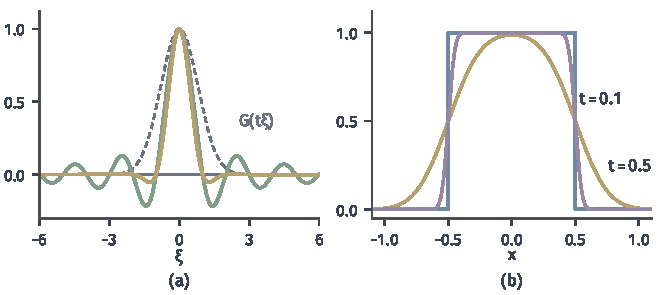
\includegraphics[width=112mm]{figures/04-spaces-measures-and-geometry/03-function-spaces/matplotlib/fourier-gauss-smoothing/figure.pdf}
  \caption{频域乘$G(t\xi)$与空间卷积$G_t$是同一运算，这里$f=B$。(a)绿色为$\widehat B$，灰色虚线为$G(t\xi)$（$t=0.5$），黄色为乘积。(b)蓝色为方框$B$，黄色与紫色为$B*G_t$，$t=0.5$与$t=0.1$；$t$越小，曲线越贴近方框。}
  \label{fig:fourier-gauss-smoothing}
\end{BookInlineFigure}

\paragraph{反演定理}

有了引理，令$t\to0$：左边在$\widehat f$可积时趋于逆变换，右边趋于$f$，反演就得到了。

\begin{theorem}[$L^1$反演定理]
\label{thm:fourier-l1-inversion}
设$f\in L^1(\mathbb R^d)$且$\widehat f\in L^1(\mathbb R^d)$。令
\begin{equation}
g(x)=\int_{\mathbb R^d}\widehat f(\xi)e^{2\pi\mathrm ix\cdot\xi}\,\mathrm d\xi ,
\label{eq:fourier-l1-inversion}
\end{equation}
则$g$是在无穷远处趋于零的连续函数，并且$f=g$几乎处处。若$f$在点$x_0$处连续，则$f(x_0)=g(x_0)$。
\end{theorem}

\begin{proof}
换元$\xi\mapsto-\xi$可知$g$是可积函数$\xi\mapsto\widehat f(-\xi)$的Fourier变换，由定理~\ref{thm:fourier-l1-properties}，它连续且在无穷远处趋于零。

在式~\eqref{eq:fourier-gauss-regularized}中令$t\to0$。左边的被积函数逐点趋于$\widehat f(\xi)e^{2\pi\mathrm ix\cdot\xi}$，并被可积函数$\lvert\widehat f\rvert$控制，所以左边对每个$x$趋于$g(x)$。

另一方面，引理~\ref{lem:fourier-gauss-approx}第2条说明$f*G_t\to f$于$L^1$。按$L^1$收敛的序列有几乎处处收敛的子列（第~\ref{chap:function-normed-spaces}章），所以沿某个子列$t_n\to0$，$(f*G_{t_n})(x)\to f(x)$对几乎每个$x$成立。两个极限相等，故$f=g$几乎处处。

若$f$在$x_0$处连续，对$\varepsilon>0$取$r>0$，使$\lvert x-x_0\rvert<r$时
\[
\lvert f(x)-f(x_0)\rvert<\varepsilon,\qquad\lvert g(x)-g(x_0)\rvert<\varepsilon.
\]
这个球的测度为正，其中有点$x$满足$f(x)=g(x)$，所以$\lvert f(x_0)-g(x_0)\rvert<2\varepsilon$。由$\varepsilon$任意，得到$f(x_0)=g(x_0)$。
\end{proof}

定理有三层含义。第一，反演公式给出的是$f$的一个连续代表，原函数作为等价类与它相等。第二，凡是$\widehat f$可积的$f$，必与一个连续函数几乎处处相等；方框有跳跃，所以$\widehat B$不可积，这与前面的直接计算一致。第三，变换是单射：若$\widehat f=\widehat g$，则$\widehat{f-g}=0$可积，反演给出$f=g$几乎处处，这相当于有限维中“坐标全同则向量相同”。

双边指数满足定理的条件，而且处处连续，所以反演对每个$x$成立：
\[
e^{-\lvert x\rvert}=\int_{\mathbb R}\frac{2}{1+4\pi^2\xi^2}\,e^{2\pi\mathrm ix\xi}\,\mathrm d\xi.
\]
在$x=0$处检验。作换元$u=2\pi\xi$，右边变成
\[
\int_{\mathbb R}\frac{2}{1+4\pi^2\xi^2}\,\mathrm d\xi=\frac1\pi\int_{\mathbb R}\frac{\mathrm du}{1+u^2}=1,
\]
与左边的$e^0=1$一致。

\paragraph{逐点反演与对称截断}

$\widehat f$不可积时，式~\eqref{eq:fourier-inverse}只能理解为某种极限。一维中最常用的是对称截断。对有限的$R$，积分区间有界，Fubini定理可用，内层积分算出来是
\[
\int_{-R}^{R}e^{2\pi\mathrm i(x-y)\xi}\,\mathrm d\xi=\frac{\sin\bigl(2\pi R(x-y)\bigr)}{\pi(x-y)}.
\]
再换元$t=x-y$，得到
\begin{equation}
\int_{-R}^{R}\widehat f(\xi)e^{2\pi\mathrm ix\xi}\,\mathrm d\xi=\int_{\mathbb R}f(x-t)\,\frac{\sin(2\pi Rt)}{\pi t}\,\mathrm dt .
\label{eq:fourier-symmetric-truncation}
\end{equation}
这里的核$\sin(2\pi Rt)/(\pi t)$扮演Dirichlet核的角色。下面需要它的积分，也就是Dirichlet积分
\[
\int_0^\infty\frac{\sin s}{s}\,\mathrm ds=\frac\pi2.
\]

Dirichlet积分可以用周期情形的工具算出。由$\frac1{2\pi}\int_0^\pi D_N=\frac12$和式~\eqref{eq:fourier-dirichlet-closed}，得到
\[
\int_0^\pi\frac{\sin\bigl((N+\tfrac12)t\bigr)}{\sin(t/2)}\,\mathrm dt=\pi.
\]
函数$\frac1{\sin(t/2)}-\frac2t$在$(0,\pi]$上有界（$t\to0$时趋于零），由Riemann--Lebesgue引理，把分母换成$t/2$不改变极限。作换元$s=(N+\tfrac12)t$，于是
\[
\lim_{N\to\infty}\int_0^{(N+1/2)\pi}\frac{\sin s}{s}\,\mathrm ds=\frac\pi2.
\]
反常积分$\int_0^\infty\frac{\sin s}{s}\,\mathrm ds$由分部积分知收敛，极限沿这个子列读出，就是$\pi/2$。

\begin{theorem}[对称截断的逐点反演]
\label{thm:fourier-symmetric-inversion}
设$f\in L^1(\mathbb R)$，并且在每个有界区间上都是分段$C^1$的。则对每个$x$，
\begin{equation}
\lim_{R\to\infty}\int_{-R}^{R}\widehat f(\xi)e^{2\pi\mathrm ix\xi}\,\mathrm d\xi=\frac{f(x+)+f(x-)}2 .
\label{eq:fourier-symmetric-inversion}
\end{equation}
\end{theorem}

\begin{proof}
核$\sin(2\pi Rt)/(\pi t)$是偶函数，所以式~\eqref{eq:fourier-symmetric-truncation}的右边可以写成$(0,\infty)$上的积分，被积函数含$f(x+t)+f(x-t)$。把积分在$t=1$处分开，并在$(0,1)$上减去左右极限，得到三项：
\[
\begin{aligned}
&\int_1^\infty\frac{f(x+t)+f(x-t)}{\pi t}\sin(2\pi Rt)\,\mathrm dt\\
&\quad+\int_0^1\frac{h(t)}{\pi t}\sin(2\pi Rt)\,\mathrm dt\\
&\quad+\bigl(f(x+)+f(x-)\bigr)\int_0^1\frac{\sin(2\pi Rt)}{\pi t}\,\mathrm dt,
\end{aligned}
\]
其中$h(t)=f(x+t)-f(x+)+f(x-t)-f(x-)$。

第一项的被积系数在$(1,\infty)$上可积，因为$f\in L^1$且$1/t\leq1$。第二项的被积系数在$(0,1)$上有界：靠近$t=0$处用定理~\ref{thm:fourier-dirichlet}证明中的单侧Lipschitz估计，其余部分用$f$在有界区间上有界。由引理~\ref{lem:fourier-riemann-lebesgue}，这两项都趋于零。

第三项作换元$s=2\pi Rt$，由Dirichlet积分，得到
\[
\int_0^1\frac{\sin(2\pi Rt)}{\pi t}\,\mathrm dt=\frac1\pi\int_0^{2\pi R}\frac{\sin s}{s}\,\mathrm ds\to\frac12.
\]
\end{proof}

对方框$B$，这一结论在$x=\pm1/2$处给出$1/2$，在其余点给出$B(x)$，这是Dirichlet定理在全空间上的对应结果。

本节的两个问题要分开看待。变换的存在只需要$f\in L^1$，在每个频率处都有确定的值。反演则另需条件：$\widehat f\in L^1$时反演积分绝对收敛，结论在几乎处处意义下成立；只有局部正则性时，要先规定积分的极限方式，结论在每一点成立，跳跃点处得到平均值。

\section{\texorpdfstring{$L^2$}{L2}中的Fourier变换}
\label{sec:fourier-l2}

周期情形的Parseval关系是无限维的勾股定理。全空间上我们也希望有$\int\lvert f\rvert^2=\int\lvert\widehat f\rvert^2$这样的等式，让Fourier变换像酉矩阵一样保持长度。但这个等式属于$L^2$，而上一节的积分定义要求$f\in L^1$。

在$\mathbb R$上两个空间互不包含，反例如下。$s(x)=\sin(\pi x)/(\pi x)$平方可积却不绝对可积，它的不可积性上一节已经算过。另一方面，函数
\[
u(x)=\lvert x\rvert^{-1/2}\mathbf 1_{\{0<\lvert x\rvert<1\}}
\]
绝对可积，$\int u=4$，却不平方可积，因为$\int_{-1}^1\lvert x\rvert^{-1}\,\mathrm dx$发散。

路线与从有理数造实数相同：在交集$L^1\cap L^2$上用原积分定义变换，证明它保持$L^2$范数，再借助稠密性把它延拓到整个$L^2$。在实轴上，$\sqrt2$不能写成有理数，但它是有理数列的极限；一个$L^2$函数也许无法直接积分，但它是$L^1\cap L^2$中函数的极限。

\paragraph{截取逼近}

延拓之前先确认$L^1\cap L^2$在$L^2$中稠密。对$f\in L^2(\mathbb R^d)$，同时截去远处与过大的取值：
\[
f_n=f\,\mathbf 1_{\{\lvert x\rvert\leq n,\ \lvert f(x)\rvert\leq n\}},\qquad n=1,2,\ldots .
\]
$f_n$的支撑含于半径$n$的球中，取值不超过$n$，所以$f_n$可积。又$\lvert f_n\rvert\leq\lvert f\rvert$，所以$f_n\in L^1\cap L^2$。

对几乎每个$x$，$f(x)$有限，当$n\geq\max\{\lvert x\rvert,\lvert f(x)\rvert\}$时$f_n(x)=f(x)$，所以$\lvert f_n-f\rvert^2\to0$几乎处处。又$\lvert f_n-f\rvert^2\leq\lvert f\rvert^2$可积，由控制收敛定理，
\[
\lVert f_n-f\rVert_2\to0.
\]

用一个例子看截断的量。取$g(x)=1/(1+\lvert x\rvert)$，它平方可积（$\int g^2=2$），但$\int g$发散。这时$g\leq1$，只需截去远处，令$g_n=g\mathbf 1_{\{\lvert x\rvert\leq n\}}$，尾部的能量是
\[
\lVert g-g_n\rVert_2^2=2\int_n^\infty\frac{\mathrm dx}{(1+x)^2}=\frac2{1+n}.
\]
$n=1,9,99$时依次为$1$、$0.2$、$0.02$，虽然慢，但趋于零。

同一截取还给出$L^2$中的平移连续性：$y\to0$时$\lVert\tau_yf-f\rVert_2\to0$。论证与引理~\ref{lem:fourier-fejer}的证明相同。$f_n$有界且可积，所以
\[
\lVert\tau_yf_n-f_n\rVert_2^2\leq2n\,\lVert\tau_yf_n-f_n\rVert_1\to0.
\]
而平移保持$L^2$范数，于是
\[
\lVert\tau_yf-f\rVert_2\leq2\lVert f-f_n\rVert_2+\lVert\tau_yf_n-f_n\rVert_2.
\]

\begin{lemma}[$L^2$中的Gauss光滑化]
\label{lem:fourier-gauss-l2}
设$f\in L^2(\mathbb R^d)$，$t>0$。则$f*G_t$对每个$x$有定义，属于$L^2(\mathbb R^d)$，并且$t\to0$时$\lVert f*G_t-f\rVert_2\to0$。若还有$f\in L^1(\mathbb R^d)$，则$f*G_t\in L^1(\mathbb R^d)$且
\begin{equation}
\widehat{f*G_t}(\xi)=\widehat f(\xi)\,G(t\xi).
\label{eq:fourier-gauss-l2-product}
\end{equation}
\end{lemma}

\begin{proof}
由Cauchy--Schwarz不等式，
\[
\int\lvert f(y)\rvert G_t(x-y)\,\mathrm dy\leq\lVert f\rVert_2\lVert G_t\rVert_2,
\]
所以卷积处处有定义。

$G_t(h)\,\mathrm dh$是概率测度，再用一次Cauchy--Schwarz不等式，得到
\[
\lvert(f*G_t)(x)-f(x)\rvert^2\leq\int G_t(h)\lvert f(x-h)-f(x)\rvert^2\,\mathrm dh.
\]
对$x$积分，交换次序，再换元$h=tu$，于是
\[
\lVert f*G_t-f\rVert_2^2\leq\int G(u)\lVert\tau_{tu}f-f\rVert_2^2\,\mathrm du.
\]
被积函数不超过$4\lVert f\rVert_2^2G(u)$，右边有限，所以$f*G_t-f\in L^2$，从而$f*G_t\in L^2$。由平移连续性与控制收敛定理，右边在$t\to0$时趋于零。

若$f\in L^1$，Tonelli定理给出$\lVert f*G_t\rVert_1\leq\lVert f\rVert_1$。再用Fubini定理与换元$z=x-y$，得到
\[
\widehat{f*G_t}(\xi)=\int f(y)e^{-2\pi\mathrm iy\cdot\xi}\Bigl(\int G_t(z)e^{-2\pi\mathrm iz\cdot\xi}\,\mathrm dz\Bigr)\mathrm dy=\widehat f(\xi)\,\widehat{G_t}(\xi).
\]
换元$z=tu$给出$\widehat{G_t}(\xi)=\widehat G(t\xi)=G(t\xi)$。
\end{proof}

式~\eqref{eq:fourier-gauss-l2-product}是第~\ref{sec:fourier-operations}节卷积规则的一个特例，这里要用到它，所以直接验证。

\subsection{等距延拓}
\label{sec:fourier-l2-extension}

\paragraph{交集上的Plancherel恒等式}

先在一个更小的集合上证明能量关系，那里所有积分都绝对收敛。记
\[
D=\{f\in L^1\cap L^2:\widehat f\in L^1\}.
\]
对$f\in D$，$\widehat f$有界且可积，所以也平方可积；由定理~\ref{thm:fourier-l1-inversion}，$f$几乎处处等于$\widehat f$的逆变换。把一个$f$换成反演公式，再交换积分次序，就得到
\[
\begin{aligned}
\int\lvert f\rvert^2\,\mathrm dx
&=\int\overline{f(x)}\Bigl(\int\widehat f(\xi)e^{2\pi\mathrm ix\cdot\xi}\,\mathrm d\xi\Bigr)\mathrm dx\\
&=\int\widehat f(\xi)\,\overline{\int f(x)e^{-2\pi\mathrm ix\cdot\xi}\,\mathrm dx}\,\mathrm d\xi\\
&=\int\lvert\widehat f\rvert^2\,\mathrm d\xi .
\end{aligned}
\]
交换次序的依据是二重积分绝对收敛，其值为$\lVert f\rVert_1\lVert\widehat f\rVert_1<\infty$。

\begin{theorem}[Plancherel恒等式]
\label{thm:fourier-plancherel-l1l2}
若$f\in L^1(\mathbb R^d)\cap L^2(\mathbb R^d)$，则$\widehat f\in L^2(\mathbb R^d)$，并且
\begin{equation}
\lVert\widehat f\rVert_2=\lVert f\rVert_2 .
\label{eq:fourier-plancherel-l1l2}
\end{equation}
\end{theorem}

\begin{proof}
一般的$f$未必属于$D$，用Gauss光滑化把它变成$D$中的元素。令$f_t=f*G_t$。由引理~\ref{lem:fourier-gauss-l2}，$f_t\in L^1\cap L^2$，且$\widehat{f_t}=\widehat f\,G(t\,\cdot)$。$\widehat f$有界、$G(t\,\cdot)$可积，所以$\widehat{f_t}\in L^1$，即$f_t\in D$。

对$f_t$用上面的恒等式，并注意$G(t\xi)^2=e^{-2\pi t^2\lvert\xi\rvert^2}$，得到
\[
\int\lvert\widehat f(\xi)\rvert^2e^{-2\pi t^2\lvert\xi\rvert^2}\,\mathrm d\xi=\lVert f_t\rVert_2^2.
\]
令$t\downarrow0$。左边的被积函数单调增加到$\lvert\widehat f\rvert^2$，由单调收敛定理，左边趋于$\int\lvert\widehat f\rvert^2$。右边由引理~\ref{lem:fourier-gauss-l2}趋于$\lVert f\rVert_2^2$。
\end{proof}

用方框核对。$\lVert B\rVert_2^2=1$，定理说$\int(\sin\pi\xi/(\pi\xi))^2\,\mathrm d\xi=1$。这个积分用初等方法并不好算，下面还会用反演另外验证。

\paragraph{延拓到$L^2$}

现在$f\mapsto\widehat f$是稠密子空间$L^1\cap L^2$到完备空间$L^2$的线性等距映射。第~\ref{chap:metric-space-maps}章证明了：稠密子集上的一致连续映射，若目标空间完备，就有唯一的连续延拓，并且Lipschitz常数保持不变。把它用于这一等距映射，就得到通常所说的\term{Plancherel定理}（Plancherel theorem）。

\begin{theorem}[Plancherel定理]
\label{thm:fourier-plancherel}
存在唯一的连续映射$\mathcal F:L^2(\mathbb R^d)\to L^2(\mathbb R^d)$，使$\mathcal Ff=\widehat f$对$f\in L^1\cap L^2$成立。$\mathcal F$是线性等距：$\lVert\mathcal Ff\rVert_2=\lVert f\rVert_2$。对任意$f\in L^2$，下式在$L^2$范数下成立：
\begin{equation}
\mathcal Ff=\lim_{n\to\infty}\int_{\lvert x\rvert\leq n}f(x)e^{-2\pi\mathrm ix\cdot(\cdot)}\,\mathrm dx .
\label{eq:fourier-plancherel-limit}
\end{equation}
\end{theorem}

\begin{proof}
存在性与唯一性由上述延拓定理给出。

等距性：对$f\in L^2$取$g_n\in L^1\cap L^2$，$g_n\to f$，由$\mathcal F$的连续性与式~\eqref{eq:fourier-plancherel-l1l2}，得到
\[
\lVert\mathcal Ff\rVert_2=\lim_n\lVert\widehat{g_n}\rVert_2=\lim_n\lVert g_n\rVert_2=\lVert f\rVert_2.
\]
线性同样由$L^1\cap L^2$上的线性取极限得到。

最后，$f\mathbf 1_{\{\lvert x\rvert\leq n\}}$在有限测度的球上平方可积，由Cauchy--Schwarz不等式也可积，并在$L^2$中收敛到$f$，所以它们的变换收敛到$\mathcal Ff$。
\end{proof}

此后对$f\in L^2$也写$\widehat f=\mathcal Ff$，称为$f$的Fourier变换；在$L^1\cap L^2$上，这一记号与原积分定义一致。

\paragraph{频域元素是等价类}

延拓得到的$\mathcal Ff$是$L^2$中的元素，即几乎处处相等的函数组成的等价类，不是一个在每个频率处都有确定值的函数。对一般的$f\in L^2$，积分$\int f(x)e^{-2\pi\mathrm ix\cdot\xi}\,\mathrm dx$不必绝对收敛，式~\eqref{eq:fourier-plancherel-limit}的极限也只在范数意义下成立，不保证对某个固定的$\xi$收敛。

例如$s(x)=\sin(\pi x)/(\pi x)$平方可积而不绝对可积，对它不能用定义~\ref{def:fourier-transform-l1}在任何一个频率处读取变换。下一小节将算出$\mathcal Fs=\mathbf 1_{[-1/2,1/2]}$，这是$L^2$中的等式，频率$\pm1/2$处的值没有意义，正如改变方框在端点的取值不改变它所代表的元素。这与$L^1$情形形成对照：那里$\widehat f$是处处有定义的连续函数，可以在单个频率处求值。

\subsection{\texorpdfstring{$L^2$}{L2}反演与Parseval关系}
\label{sec:fourier-l2-inversion}

\paragraph{反演与内积保持}

在$L^2$中，反演有一个干净的形式。记反射$(Rf)(x)=f(-x)$，它是$L^2$上的等距。对$f\in L^1$，直接换元得到
\[
\widehat{Rf}(\xi)=\int f(-x)e^{-2\pi\mathrm ix\cdot\xi}\,\mathrm dx=\widehat f(-\xi).
\]
两边都连续地依赖$f$，所以$\mathcal FR=R\mathcal F$在$L^2$上成立。逆变换式~\eqref{eq:fourier-inverse}恰为$\check h=R\widehat h$，因此它延拓到$L^2$后的映射就是$R\mathcal F$。

\begin{theorem}[$L^2$反演与Parseval关系]
\label{thm:fourier-l2-inversion}
$\mathcal F$是$L^2(\mathbb R^d)$到自身的双射，逆映射为$\mathcal F^{-1}=R\mathcal F$，并且$\mathcal F\mathcal F=R$。对任意$f,g\in L^2(\mathbb R^d)$，
\begin{equation}
\int_{\mathbb R^d}\overline{f(x)}\,g(x)\,\mathrm dx=\int_{\mathbb R^d}\overline{\widehat f(\xi)}\,\widehat g(\xi)\,\mathrm d\xi .
\label{eq:fourier-l2-parseval}
\end{equation}
\end{theorem}

\begin{proof}
先证$R\mathcal F\mathcal F=I$。对$f\in D$，$\widehat f\in L^1\cap L^2$，所以$R\mathcal F(\widehat f)$可以用积分计算，它就是$\widehat f$的逆变换，由定理~\ref{thm:fourier-l1-inversion}等于$f$。所以$R\mathcal F\mathcal F=I$在$D$上成立。

定理~\ref{thm:fourier-plancherel-l1l2}的证明表明，每个$f\in L^1\cap L^2$都是$D$中元素$f*G_t$的$L^2$极限，而$L^1\cap L^2$在$L^2$中稠密，所以$D$在$L^2$中稠密。两边都是连续映射，故$R\mathcal F\mathcal F=I$在$L^2$上成立。

由$R^2=I$得$\mathcal F\mathcal F=R$。再由$\mathcal FR=R\mathcal F$得$\mathcal F(R\mathcal F)=R\mathcal F\mathcal F=I$。所以$\mathcal F$是双射，逆为$R\mathcal F$。

内积保持来自范数保持。对第二个变量线性的复内积，由范数表示的公式是
\[
\langle f,g\rangle=\frac14\sum_{k=0}^3\mathrm i^{-k}\lVert f+\mathrm i^kg\rVert_2^2.
\]
$\mathcal F$线性且保持每个$f+\mathrm i^kg$的范数，所以保持内积。
\end{proof}

这就是有限维酉矩阵的全部性质：保持长度和内积，逆等于“共轭转置”。把$\mathcal F$作用两次等于反射，这一点第~\ref{sec:fourier-discrete}节会用$4\times4$矩阵具体看到。式~\eqref{eq:fourier-l2-parseval}是全空间上的Parseval关系，取$g=f$即能量关系$\lVert\widehat f\rVert_2=\lVert f\rVert_2$，在本章的归一化下两边没有额外常数。

现在可以算出$\mathcal Fs$。方框$B$属于$L^1\cap L^2$，$\widehat B=s$。由$\mathcal F\mathcal F=R$，并注意$B$是偶函数，得到
\[
\mathcal Fs=\mathcal F\mathcal FB=RB=B.
\]
能量关系同时给出
\[
\int_{\mathbb R}\Bigl(\frac{\sin\pi x}{\pi x}\Bigr)^2\,\mathrm dx=\lVert B\rVert_2^2=1.
\]

\paragraph{同一公式的不同含义}

反演公式~\eqref{eq:fourier-l1-inversion}在本章出现了三次，含义各不相同，表~\ref{tab:fourier-inversion-meanings}把它们并列。把积分区域限制在$\lvert\xi\rvert\leq R$得到的截断积分，是否对几乎每个$x$逐点收敛，是深刻得多的问题，本书不讨论。

\begin{BookInlineTable}
  \centering
  \small
  \begin{tabular}{@{}lll@{}}
    \toprule
    条件 & 右边的含义 & 等式的意义\\
    \midrule
    $f,\widehat f\in L^1$ & 绝对收敛的积分 & 几乎处处；连续点处逐点\\
    一维，局部分段$C^1$ & 对称截断的极限 & 每一点；跳跃点取平均\\
    $f\in L^2$ & 截断积分的$L^2$极限 & 范数意义\\
    \bottomrule
  \end{tabular}
  \caption{反演公式在三种条件下的含义。}
  \label{tab:fourier-inversion-meanings}
\end{BookInlineTable}

\paragraph{归一化与常数}

不同文献的Fourier变换只差自变量伸缩与常数因子，但反演与能量公式中的常数必须与定义配套。表~\ref{tab:fourier-normalizations}比较三种常见约定，其中第二、三行用角频率$\omega=2\pi\xi$。

\begin{BookInlineTable}
  \centering
  \small
  \begin{tabularx}{\linewidth}{@{}>{\raggedright\arraybackslash}p{20mm}>{\raggedright\arraybackslash}X>{\raggedright\arraybackslash}p{28mm}@{}}
    \toprule
    约定 & 正变换与反变换 & 能量关系\\
    \midrule
    频率$\xi$（本章） & $\widehat f(\xi)=\int fe^{-2\pi\mathrm ix\cdot\xi}\,\mathrm dx$，$f=\int\widehat fe^{2\pi\mathrm ix\cdot\xi}\,\mathrm d\xi$ & $\int\lvert f\rvert^2=\int\lvert\widehat f\rvert^2$\\
    角频率，正变换不加因子 & $F(\omega)=\int fe^{-\mathrm ix\cdot\omega}\,\mathrm dx$，$f=(2\pi)^{-d}\int Fe^{\mathrm ix\cdot\omega}\,\mathrm d\omega$ & $\int\lvert f\rvert^2=(2\pi)^{-d}\int\lvert F\rvert^2$\\
    角频率，对称归一 & 正、反变换各乘$(2\pi)^{-d/2}$ & $\int\lvert f\rvert^2=\int\lvert F\rvert^2$\\
    \bottomrule
  \end{tabularx}
  \caption{$\mathbb R^d$上Fourier变换的三种常见归一化。各行之间的换算是$F(\omega)=\widehat f(\omega/2\pi)$，对称归一化再乘以$(2\pi)^{-d/2}$；所有结论只差这些常数。}
  \label{tab:fourier-normalizations}
\end{BookInlineTable}

以第二行为例核对常数。作换元$\omega=2\pi\xi$，$\mathrm d\omega=(2\pi)^d\,\mathrm d\xi$，得到
\[
\int\lvert F(\omega)\rvert^2\,\mathrm d\omega=\int\lvert\widehat f(\omega/2\pi)\rvert^2\,\mathrm d\omega=(2\pi)^d\int\lvert\widehat f(\xi)\rvert^2\,\mathrm d\xi,
\]
所以能量关系中出现$(2\pi)^{-d}$。周期情形同样如此：第~\ref{sec:fourier-series}节把$1/(2\pi)$放进内积，Parseval关系才不含常数。

\section{Fourier变换下的运算}
\label{sec:fourier-operations}

有限维中，对称矩阵在特征向量基下变成对角矩阵，矩阵的作用只是把每个坐标乘一个数。平面波$e_\xi(x)=e^{2\pi\mathrm ix\cdot\xi}$对几种基本运算扮演同样的角色。平移$a$之后，
\[
e_\xi(x-a)=e^{-2\pi\mathrm ia\cdot\xi}\,e_\xi(x),
\]
求导之后，
\[
\partial_je_\xi=2\pi\mathrm i\xi_j\,e_\xi .
\]
所以每个平面波都是平移和求导的公共“特征向量”，而特征值是$\xi$的已知函数。这就是频率坐标好用的根本原因：这些运算在频率坐标下都是对角的。

这一说法只是启发。平面波不属于$L^1$，也不属于$L^2$，上面的“特征向量”并不在所讨论的空间里，所以每条规则都要用换元、分部积分或交换积分次序实际证明，而每一步都有前提。本节对每条规则先在$L^1(\mathbb R^d)$中给出证明，再说明它在什么条件下推广到$L^2$，所用的卷积与弱导数来自第~\ref{chap:smoothing-weak-derivatives}章。

\subsection{平移}
\label{sec:fourier-translation}

把函数整体移动$a\in\mathbb R^d$，记$(\tau_af)(x)=f(x-a)$。按上面的特征值，平移不应改变各频率成分的大小，只改变它们的相位。与之对偶的操作是乘以平面波，记$(M_bf)(x)=e^{2\pi\mathrm ib\cdot x}f(x)$，称为\term{调制}（modulation）。

\begin{theorem}[平移与调制]
\label{thm:fourier-translation}
设$f\in L^1(\mathbb R^d)$，$a,b\in\mathbb R^d$。则对每个$\xi$，
\begin{equation}
\widehat{\tau_af}(\xi)=e^{-2\pi\mathrm ia\cdot\xi}\,\widehat f(\xi),\qquad\widehat{M_bf}(\xi)=\widehat f(\xi-b).
\label{eq:fourier-translation}
\end{equation}
两式对$f\in L^2(\mathbb R^d)$在$L^2$意义下同样成立。
\end{theorem}

\begin{proof}
第一式作换元$x=y+a$：
\[
\int f(x-a)e^{-2\pi\mathrm ix\cdot\xi}\,\mathrm dx=\int f(y)e^{-2\pi\mathrm i(y+a)\cdot\xi}\,\mathrm dy=e^{-2\pi\mathrm ia\cdot\xi}\widehat f(\xi).
\]
第二式只需把两个指数合并成$e^{-2\pi\mathrm ix\cdot(\xi-b)}$。

对$L^2$，四个映射$f\mapsto\tau_af$、$f\mapsto M_bf$、乘以$e^{-2\pi\mathrm ia\cdot\xi}$、频率平移$b$都是$L^2$上的等距，$\mathcal F$也是。所以两边作为$f$的映射都连续，又在稠密子空间$L^1\cap L^2$上相等，因而在$L^2$上相等。
\end{proof}

两条规则方向相反，不能混淆。函数平移产生频率上的相位因子，频谱的大小$\lvert\widehat f\rvert$不变，完全看不出平移量；频率平移则来自函数上的相位因子。指数的符号取决于定义中的约定。周期情形有同样的规则，第$k$个坐标乘以$e^{-\mathrm ika}$，证明也是换元。

用$\mathbf 1_{[0,1]}=\tau_{1/2}B$作一个核对。平移规则与式~\eqref{eq:fourier-box}给出
\[
\widehat{\mathbf 1_{[0,1]}}(\xi)=e^{-\pi\mathrm i\xi}\,\frac{\sin\pi\xi}{\pi\xi}.
\]
直接积分得到$\frac{1-e^{-2\pi\mathrm i\xi}}{2\pi\mathrm i\xi}$，提出因子$e^{-\pi\mathrm i\xi}$后，
\[
\frac{1-e^{-2\pi\mathrm i\xi}}{2\pi\mathrm i\xi}=e^{-\pi\mathrm i\xi}\,\frac{e^{\pi\mathrm i\xi}-e^{-\pi\mathrm i\xi}}{2\pi\mathrm i\xi}=e^{-\pi\mathrm i\xi}\,\frac{\sin\pi\xi}{\pi\xi},
\]
两者一致。

\subsection{缩放}
\label{sec:fourier-scaling}

把自变量乘以$\lambda>1$，函数在空间中被压窄。频率的含义是单位长度内的圈数，压窄后同样的振荡出现在更短的长度上，频率应当按$\lambda$放大；同时积分区域缩小，幅度要乘以一个Jacobian因子。下面对一般的可逆线性变换推导这一点。

\begin{theorem}[线性变量替换]
\label{thm:fourier-scaling}
设$f\in L^1(\mathbb R^d)$，$\bm A$是$d\times d$可逆实矩阵。则
\begin{equation}
\widehat{f\circ\bm A}(\xi)=\frac1{\lvert\det\bm A\rvert}\,\widehat f\bigl(\bm A^{-\top}\xi\bigr).
\label{eq:fourier-linear-change}
\end{equation}
特别地，对实数$\lambda\neq0$，
\begin{equation}
\widehat{f(\lambda\,\cdot)}(\xi)=\lvert\lambda\rvert^{-d}\,\widehat f(\xi/\lambda).
\label{eq:fourier-scaling}
\end{equation}
\end{theorem}

\begin{proof}
作换元$y=\bm Ax$。Lebesgue测度在线性变换下乘以$\lvert\det\bm A\rvert$，即$\mathrm dx=\lvert\det\bm A\rvert^{-1}\mathrm dy$（第~\ref{chap:integration}章）。指数中的内积变成
\[
x\cdot\xi=(\bm A^{-1}y)\cdot\xi=y\cdot(\bm A^{-\top}\xi).
\]
代入定义，于是
\[
\int f(\bm Ax)e^{-2\pi\mathrm ix\cdot\xi}\,\mathrm dx=\frac1{\lvert\det\bm A\rvert}\int f(y)e^{-2\pi\mathrm iy\cdot\bm A^{-\top}\xi}\,\mathrm dy.
\]
取$\bm A=\lambda\bm I$，$\det\bm A=\lambda^d$，$\bm A^{-\top}\xi=\xi/\lambda$，就是第二式。
\end{proof}

公式中三个量各有来源。频率尺度$\xi/\lambda$说明：$\lambda>1$时原函数压窄，变换展宽。因子$\lvert\lambda\rvert^{-d}$是Jacobian，它随维数$d$改变；各坐标分别按$\lambda_1,\ldots,\lambda_d$缩放时，因子为$\prod_i\lvert\lambda_i\rvert^{-1}$，第$i$个频率坐标变为$\xi_i/\lambda_i$。转置逆$\bm A^{-\top}$说明频率按对偶方式变换：旋转在频域中仍是同一个旋转，剪切则不然。

图~\ref{fig:fourier-scaling}取$\lambda=1/2$。方框加宽一倍，式~\eqref{eq:fourier-scaling}给出
\[
\widehat{B(\cdot/2)}(\xi)=2\,\widehat B(2\xi)=\frac{\sin(2\pi\xi)}{\pi\xi},
\]
与上一节的直接计算一致。空间中变宽，频域中变窄；中央的高度翻倍，因为$\xi=0$处的值就是函数的积分，$\int B(x/2)\,\mathrm dx=2$。

\begin{BookInlineFigure}
  \centering
  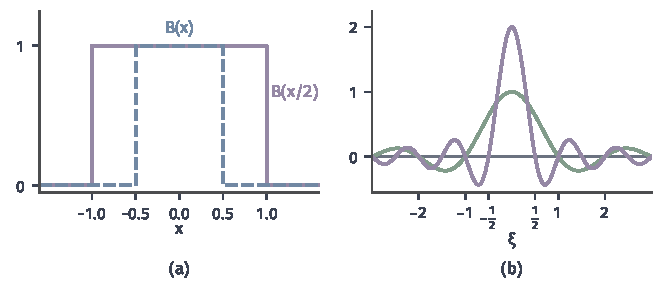
\includegraphics[width=112mm]{figures/04-spaces-measures-and-geometry/03-function-spaces/matplotlib/fourier-scaling/figure.pdf}
  \caption{缩放的对偶。(a)蓝色虚线为方框$B(x)$，紫色为加宽一倍的$B(x/2)$。(b)绿色为$\widehat B$，第一个零点在$\xi=\pm1$；紫色为$B(x/2)$的变换，第一个零点在$\xi=\pm\frac12$，中央高度为$2$。}
  \label{fig:fourier-scaling}
\end{BookInlineFigure}

Gauss核也可以检验。$G_t=t^{-d}G(\cdot/t)$对应$\lambda=1/t$，公式给出
\[
\widehat{G_t}(\xi)=t^{-d}\cdot t^d\,\widehat G(t\xi)=G(t\xi),
\]
正是反演证明中用到的等式。

在$L^2$中常用保持范数的伸缩
\[
D_\lambda f=\lvert\lambda\rvert^{d/2}f(\lambda\,\cdot).
\]
式~\eqref{eq:fourier-scaling}给出$\widehat{D_\lambda f}=D_{1/\lambda}\widehat f$。两边都是$L^2$上的等距，在$L^1\cap L^2$上相等，所以在$L^2$上相等。这一归一化把Jacobian因子平分到两侧，第~\ref{chap:wavelet-transform}章的小波伸缩采用同样的写法。

\subsection{微分}
\label{sec:fourier-differentiation}

周期情形的分部积分给出$\widehat{f'}(k)=\mathrm ik\widehat f(k)$，边界项因周期性抵消。全空间上没有周期，边界项能否消失取决于函数在远处的行为；在函数不可导的点，还要借助弱导数。下面先处理边界项自动消失的情形，再处理一般情形。

\paragraph{光滑紧支撑函数}

设$f$连续可微且支撑紧。固定其余坐标，在一个包含支撑的有界区间上对$x_j$分部积分，边界项为零，得到
\[
\int\partial_jf(x)\,e^{-2\pi\mathrm ix\cdot\xi}\,\mathrm dx_j=-\int f(x)\,\partial_j\bigl(e^{-2\pi\mathrm ix\cdot\xi}\bigr)\,\mathrm dx_j.
\]
指数对$x_j$求导带下来因子$-2\pi\mathrm i\xi_j$，所以
\[
\int\partial_jf(x)\,e^{-2\pi\mathrm ix\cdot\xi}\,\mathrm dx_j=2\pi\mathrm i\xi_j\int f(x)e^{-2\pi\mathrm ix\cdot\xi}\,\mathrm dx_j.
\]
再对其余坐标积分（Fubini定理），得到
\[
\widehat{\partial_jf}(\xi)=2\pi\mathrm i\xi_j\,\widehat f(\xi).
\]
求导在频域中变成乘以$2\pi\mathrm i\xi_j$，与开头的特征值一致。

\paragraph{弱导数可积的情形}

一般的可积函数没有紧支撑，也未必处处可导。第~\ref{chap:smoothing-weak-derivatives}章用测试恒等式定义了弱导数：若局部可积函数$g$对所有$\varphi\in C_c^\infty(\mathbb R^d)$满足$\int f\,\partial_j\varphi=-\int g\,\varphi$，就称$g$为$f$的弱导数$\partial_jf$。要把这个恒等式用于$e^{-2\pi\mathrm ix\cdot\xi}$，需要先把它截断成紧支撑函数，再让截断半径趋于无穷，并控制截断边缘产生的项。

\begin{theorem}[微分规则]
\label{thm:fourier-derivative}
设$f\in L^1(\mathbb R^d)$，且$f$关于$x_j$的弱导数$\partial_jf$存在并属于$L^1(\mathbb R^d)$。则对每个$\xi\in\mathbb R^d$，
\begin{equation}
\widehat{\partial_jf}(\xi)=2\pi\mathrm i\xi_j\,\widehat f(\xi).
\label{eq:fourier-derivative}
\end{equation}
\end{theorem}

\begin{proof}
取光滑函数$\chi$，满足$0\leq\chi\leq1$，在$\lvert x\rvert\leq1$上等于$1$，在$\lvert x\rvert\geq2$上等于$0$；这样的截断函数由第~\ref{chap:smoothing-weak-derivatives}章的磨光构造得到。对$R>0$令
\[
\varphi_R(x)=\chi(x/R)\,e^{-2\pi\mathrm ix\cdot\xi},
\]
它的实部与虚部都是测试函数，所以测试恒等式对$\varphi_R$成立。按乘积求导，
\[
\partial_j\varphi_R(x)=\Bigl[\frac1R(\partial_j\chi)(x/R)-2\pi\mathrm i\xi_j\chi(x/R)\Bigr]e^{-2\pi\mathrm ix\cdot\xi}.
\]
代入测试恒等式，得到
\[
\begin{aligned}
\int\partial_jf(x)\chi(x/R)e^{-2\pi\mathrm ix\cdot\xi}\,\mathrm dx
={}&-\frac1R\int f(x)(\partial_j\chi)(x/R)e^{-2\pi\mathrm ix\cdot\xi}\,\mathrm dx\\
&+2\pi\mathrm i\xi_j\int f(x)\chi(x/R)e^{-2\pi\mathrm ix\cdot\xi}\,\mathrm dx .
\end{aligned}
\]
令$R\to\infty$。左边与右边第二项的被积函数分别被$\lvert\partial_jf\rvert$与$\lvert f\rvert$控制，且$\chi(x/R)\to1$，由控制收敛定理，它们分别趋于$\widehat{\partial_jf}(\xi)$与$2\pi\mathrm i\xi_j\widehat f(\xi)$。右边第一项是截断边缘的贡献，其模不超过
\[
\frac1R\sup\lvert\partial_j\chi\rvert\,\lVert f\rVert_1\to0.
\]
\end{proof}

证明中$f\in L^1$承担了控制边缘项的任务：截断函数的导数只有$1/R$大小，乘上可积的$f$后整体趋于零。这里没有要求$f$在远处逐点趋于零。

\paragraph{光滑性与衰减}

微分规则把光滑性转换为高频衰减。由定理~\ref{thm:fourier-l1-properties}，
\[
2\pi\lvert\xi_j\rvert\,\lvert\widehat f(\xi)\rvert=\lvert\widehat{\partial_jf}(\xi)\rvert\leq\lVert\partial_jf\rVert_1 .
\]
若各阶弱导数$\partial^\alpha f$（$\lvert\alpha\rvert\leq m$）都可积，逐次使用规则，得到
\[
\widehat{\partial^\alpha f}(\xi)=(2\pi\mathrm i\xi)^\alpha\,\widehat f(\xi),\qquad
(2\pi\mathrm i\xi)^\alpha=\prod_j(2\pi\mathrm i\xi_j)^{\alpha_j},
\]
所以$\lvert\widehat f(\xi)\rvert$按$\lvert\xi\rvert^{-m}$衰减。

对偶地，原函数在远处衰减得快，变换就光滑。若$f$与$x_jf$都可积，在积分号下对$\xi_j$求导（被积函数的导数被$2\pi\lvert x_jf\rvert$控制），得到
\[
\partial_{\xi_j}\widehat f=\widehat{-2\pi\mathrm ix_jf}.
\]

用双边指数核对。$f(x)=e^{-\lvert x\rvert}$在$0$处不可导，但有可积的弱导数$-\operatorname{sgn}(x)e^{-\lvert x\rvert}$。把弱导数的变换分成两段积分，得到
\[
-\frac1{1+2\pi\mathrm i\xi}+\frac1{1-2\pi\mathrm i\xi}=\frac{4\pi\mathrm i\xi}{1+4\pi^2\xi^2}.
\]
由式~\eqref{eq:fourier-double-exponential}，这恰好等于$2\pi\mathrm i\xi\,\widehat f(\xi)$，与定理一致。

方框$B$不满足定理的条件。形式地计算，
\[
2\pi\mathrm i\xi\,\widehat B(\xi)=2\mathrm i\sin(\pi\xi)=e^{\pi\mathrm i\xi}-e^{-\pi\mathrm i\xi}.
\]
它不随$\lvert\xi\rvert\to\infty$趋于零，由Riemann--Lebesgue引理不可能是可积函数的变换。它对应的是在$x=-1/2$与$x=1/2$处的两个符号相反的点质量，这正是跳跃函数的导数不能由局部可积函数表示的情形，超出了本节$L^1$的框架。

$L^2$函数的弱导数有对应的频域刻画：$f$与$\partial_jf$都属于$L^2$时，式~\eqref{eq:fourier-derivative}在$L^2$意义下成立。它是第~\ref{chap:sobolev-spaces}章用频率权刻画Sobolev空间的出发点，证明也留到那里。

\subsection{卷积}
\label{sec:fourier-convolution}

第~\ref{chap:smoothing-weak-derivatives}章对$f,g\in L^1(\mathbb R^d)$定义了卷积$(f*g)(x)=\int f(x-y)g(y)\,\mathrm dy$，证明它几乎处处有定义，并且
\[
\lVert f*g\rVert_1\leq\lVert f\rVert_1\lVert g\rVert_1.
\]

卷积是平移的加权叠加：
\[
f*g=\int g(y)\,\tau_yf\,\mathrm dy.
\]
平移在频域中是乘以相位因子，叠加之后应当得到$\widehat f$乘以$g$的相位加权和，也就是$\widehat f\,\widehat g$。在有限维的类比中，这说明卷积算子也在频率坐标下对角，第$\xi$个对角元就是$\widehat g(\xi)$。

\begin{theorem}[卷积规则]
\label{thm:fourier-convolution}
若$f,g\in L^1(\mathbb R^d)$，则对每个$\xi$，
\begin{equation}
\widehat{f*g}(\xi)=\widehat f(\xi)\,\widehat g(\xi).
\label{eq:fourier-convolution}
\end{equation}
\end{theorem}

\begin{proof}
先确认可以交换积分次序：
\[
\int\!\!\int\lvert f(x-y)\rvert\,\lvert g(y)\rvert\,\mathrm dx\,\mathrm dy=\lVert f\rVert_1\lVert g\rVert_1<\infty.
\]
由Fubini定理交换次序，再对内层换元$z=x-y$，得到
\[
\begin{aligned}
\widehat{f*g}(\xi)&=\int g(y)\Bigl(\int f(x-y)e^{-2\pi\mathrm ix\cdot\xi}\,\mathrm dx\Bigr)\mathrm dy\\
&=\int g(y)e^{-2\pi\mathrm iy\cdot\xi}\,\mathrm dy\cdot\int f(z)e^{-2\pi\mathrm iz\cdot\xi}\,\mathrm dz .
\end{aligned}
\]
\end{proof}

方框与自身的卷积是三角形。$(B*B)(x)$等于区间$[-1/2,1/2]$与$[x-1/2,x+1/2]$的重叠长度，所以
\[
(B*B)(x)=\Lambda(x)=\max\{0,1-\lvert x\rvert\}.
\]
图~\ref{fig:fourier-convolution-triangle}(a)画的是$x=0.4$的情形，重叠长度为$0.6$，正是(b)中$\Lambda(0.4)$的值。

卷积规则给出$\Lambda$的变换：
\[
\widehat\Lambda(\xi)=\Bigl(\frac{\sin\pi\xi}{\pi\xi}\Bigr)^2.
\]
它按$\xi^{-2}$衰减，是可积的，而$\Lambda$连续，所以由定理~\ref{thm:fourier-l1-inversion}，反演在每一点成立。在$x=0$处读出
\[
\int_{\mathbb R}\Bigl(\frac{\sin\pi\xi}{\pi\xi}\Bigr)^2\,\mathrm d\xi=\Lambda(0)=1,
\]
与上一节由能量关系算出的值一致。卷积使跳跃变成尖点，频域中的衰减也从$\xi^{-1}$加快到$\xi^{-2}$，图~\ref{fig:fourier-convolution-triangle}(c)中实线的旁瓣明显更小。

\begin{BookInlineFigure}
  \centering
  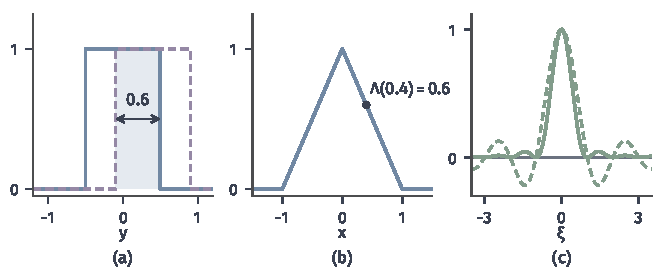
\includegraphics[width=112mm]{figures/04-spaces-measures-and-geometry/03-function-spaces/matplotlib/fourier-convolution-triangle/figure.pdf}
  \caption{方框的自卷积。(a)蓝色为$B(y)$，紫色虚线为$B(x-y)$（$x=0.4$），浅蓝色区域为重叠部分，长度$0.6$。(b)$\Lambda=B*B$，黑点对应(a)的$x$。(c)绿色虚线为$\widehat B$，绿色实线为$\widehat\Lambda=\widehat B^{\,2}$。}
  \label{fig:fourier-convolution-triangle}
\end{BookInlineFigure}

\paragraph{推广到$L^2$}

推广时要分别确认输入在哪个空间、卷积落在哪个空间、等式在什么意义下成立。

第一种情形是$f\in L^1$、$g\in L^2$。由Cauchy--Schwarz不等式，
\[
\lvert(f*g)(x)\rvert^2\leq\int\lvert f(x-y)\rvert\,\mathrm dy\cdot\int\lvert f(x-y)\rvert\,\lvert g(y)\rvert^2\,\mathrm dy.
\]
对$x$积分，得到
\[
\lVert f*g\rVert_2\leq\lVert f\rVert_1\lVert g\rVert_2,
\]
所以卷积落在$L^2$中，并且连续地依赖$g$。

此时等式$\widehat{f*g}=\widehat f\,\widehat g$在$L^2$中成立。当$g\in L^1\cap L^2$时它由定理~\ref{thm:fourier-convolution}给出。左边是$g$的连续映射，右边是乘以有界函数$\widehat f$，也连续。两边在稠密子空间上相等，所以在整个$L^2$上相等。

第二种情形是$f,g\in L^2$。此时$(f*g)(x)$对每个$x$都有定义，模不超过$\lVert f\rVert_2\lVert g\rVert_2$，由$L^2$平移连续性它还是连续函数；但它一般不属于$L^1$，也不必属于$L^2$。另一方面，$\widehat f\widehat g$作为两个$L^2$函数的乘积是可积的。因此正确的对应是逆变换，而不是$L^2$中的变换等式：
\begin{equation}
(f*g)(x)=\int_{\mathbb R^d}\widehat f(\xi)\,\widehat g(\xi)\,e^{2\pi\mathrm ix\cdot\xi}\,\mathrm d\xi\qquad\text{对每个}\ x .
\label{eq:fourier-l2-convolution}
\end{equation}

证明用Parseval关系。令$h_x(y)=f(x-y)$，则
\[
(f*g)(x)=\int h_x\,g=\langle\overline{h_x},g\rangle.
\]
由平移、反射规则，
\[
\widehat{h_x}(\xi)=e^{-2\pi\mathrm ix\cdot\xi}\widehat f(-\xi).
\]
再由共轭的规则
\[
\widehat{\overline u}(\xi)=\overline{\widehat u(-\xi)}
\]
（对$L^1$函数直接验证，再延拓到$L^2$），得到
\[
\widehat{\overline{h_x}}(\xi)=\overline{e^{2\pi\mathrm ix\cdot\xi}\widehat f(\xi)}.
\]
代入式~\eqref{eq:fourier-l2-parseval}，共轭抵消，即得式~\eqref{eq:fourier-l2-convolution}。

例如$f=g=s$时，$\widehat f\widehat g=B\cdot B=B$，式~\eqref{eq:fourier-l2-convolution}给出$s*s=s$，它平方可积却不可积。

这三种情形研究的都是Fourier变换怎样把卷积这一运算转为乘法。把卷积看作对信号的作用，讨论哪些频率被保留、哪些被削弱，属于滤波问题，在\BookChapterRef{chap:signal-systems}{卷九“信号系统”章}研究。

\section{Fourier表示与离散变换}
\label{sec:fourier-discrete}

到目前为止出现了两种频率表示：周期函数的Fourier系数是整数下标的序列，全空间函数的Fourier变换是连续频率的函数。实际计算中还有第三种：有限个数组成的向量，用有限个频率表示。三者都用复指数作坐标，但输入对象、频率集合和成立的意义都不同。本节先把三种对象并列，再说明从一种转到另一种时，需要哪些额外的约定，以及每种约定改变了什么。

\paragraph{离散Fourier变换}

有限向量的情形最简单。设$N\geq1$，把$\bm x\in\mathbb C^N$的分量记为$x[0],\ldots,x[N-1]$，并把下标看作模$N$的整数，即首尾相接。此时允许的频率只有$N$个，对应的复指数为$e^{2\pi\mathrm ikn/N}$，$k=0,\ldots,N-1$。

\begin{definition}[离散Fourier变换]
\label{def:fourier-dft}
$\bm x\in\mathbb C^N$的\term{离散Fourier变换}（discrete Fourier transform, DFT）为
\[
\widehat x[k]=\sum_{n=0}^{N-1}x[n]e^{-2\pi\mathrm ikn/N},\qquad k=0,\ldots,N-1 .
\]
\end{definition}

逆变换与能量关系都来自单位根的正交性：对整数$m$，$\sum_{n=0}^{N-1}e^{2\pi\mathrm imn/N}$在$N\mid m$时等于$N$，否则是公比$q=e^{2\pi\mathrm im/N}\neq1$且$q^N=1$的几何级数，等于$(1-q^N)/(1-q)=0$。由此
\[
x[n]=\frac1N\sum_{k=0}^{N-1}\widehat x[k]e^{2\pi\mathrm ikn/N},\qquad
\sum_{n=0}^{N-1}\lvert x[n]\rvert^2=\frac1N\sum_{k=0}^{N-1}\lvert\widehat x[k]\rvert^2 .
\]
这里所有的和都是有限和，不存在收敛问题，变换是$\mathbb C^N$上的可逆线性映射，$N^{-1/2}$倍的变换矩阵是酉矩阵。常数$1/N$的位置同样是约定，与第~\ref{sec:fourier-l2}节的表格同理。

\paragraph{三种表示的对象}

下表把三种表示并列。它们的差别首先在输入：全空间上的函数、一个周期上的函数、$N$个数。输入不同，频率集合与成立的意义也随之不同。

\begin{table}[!htb]
  \centering
  \caption{三种Fourier表示的输入对象、频率集合与成立意义。表中周期情形写成一般周期$T$，第~\ref{sec:fourier-series}节取$T=2\pi$。}
  \label{tab:fourier-three-representations}
  \small
  \begin{tabularx}{\linewidth}{@{}l>{\raggedright\arraybackslash}X>{\raggedright\arraybackslash}X>{\raggedright\arraybackslash}X@{}}
    \toprule
    表示 & 输入对象 & 频率集合 & 成立的意义\\
    \midrule
    Fourier变换 & $\mathbb R^d$上的$L^1$或$L^2$函数 & $\xi\in\mathbb R^d$ & $L^1$：处处有值；$L^2$：等价类\\
    Fourier级数 & 周期$T$的$L^1$或$L^2$函数 & $k/T$，$k\in\mathbb Z$ & $L^2$展开；逐点另需条件\\
    离散变换 & $\mathbb C^N$中的向量 & $k$，$k=0,\ldots,N-1$（模$N$） & 有限和，精确可逆\\
    \bottomrule
  \end{tabularx}
\end{table}

这三种对象不能直接互相代替。一个全空间函数没有周期，不能直接取Fourier系数；一个周期函数有无穷多个系数，不能直接作$N$点变换；$N$个数不是函数，没有连续频率。从一种表示转到另一种，必须先把对象本身转过去，下面三个操作各完成一种转换。

\paragraph{周期化：从全空间到周期}

把全空间函数变成周期函数的自然做法是把所有平移叠加起来。对$f\in L^1(\mathbb R)$，定义它的\term{周期化}（periodization）
\[
(Pf)(x)=\sum_{n\in\mathbb Z}f(x+n).
\]
由Tonelli定理，$\int_0^1\sum_n\lvert f(x+n)\rvert\,\mathrm dx=\int_{\mathbb R}\lvert f\rvert<\infty$，所以级数对几乎每个$x$绝对收敛，$Pf$以$1$为周期且在一个周期上可积。

\begin{theorem}[周期化的系数]
\label{thm:fourier-periodization}
若$f\in L^1(\mathbb R)$，则$Pf$按周期$1$计算的Fourier系数为
\[
\int_0^1(Pf)(x)e^{-2\pi\mathrm ikx}\,\mathrm dx=\widehat f(k),\qquad k\in\mathbb Z .
\]
\end{theorem}

\begin{proof}
上面的绝对收敛估计允许交换求和与积分。$e^{-2\pi\mathrm ikx}$以$1$为周期，所以
\begin{equation*}
\begin{aligned}
\int_0^1\sum_nf(x+n)e^{-2\pi\mathrm ikx}\,\mathrm dx&=\sum_n\int_n^{n+1}f(y)e^{-2\pi\mathrm iky}\,\mathrm dy\\
&=\int_{\mathbb R}f(y)e^{-2\pi\mathrm iky}\,\mathrm dy .
\end{aligned}
\end{equation*}
\end{proof}

定理说明，周期化后的Fourier系数恰是原变换在整数频率上的取值，连续频率被取样成了离散频率。代价在原函数一侧：$Pf$把相距整数的各段叠在一起。若$f$支撑在长度不超过$1$的区间内，各段不重叠，$Pf$在一个周期上就是$f$，没有信息损失；否则不同位置的值混在一起，由$Pf$不能还原$f$。以$f=e^{-\lvert x\rvert}$为例，$Pf$的系数为$2/(1+4\pi^2k^2)$，而$Pf$本身在每一点都叠加了无穷多个平移。由这一系数等式还可以得到逐点的Poisson求和公式$\sum_nf(n)=\sum_k\widehat f(k)$，但那需要额外的正则性，这里不展开。

\paragraph{取样：从周期函数到有限向量}

把周期函数变成$N$个数的自然做法是在一个周期内等距取样。设$g$以$1$为周期，Fourier系数$\widehat g(m)=\int_0^1g(x)e^{-2\pi\mathrm imx}\,\mathrm dx$绝对可和；由定理~\ref{thm:fourier-uniform}（换成周期$1$），二次连续可微就足够。此时Fourier级数一致收敛到$g$，在每一点成立。取样$x[n]=g(n/N)$，$n=0,\ldots,N-1$。

\begin{theorem}[取样的离散变换]
\label{thm:fourier-sampling-aliasing}
在上述条件下，
\[
\widehat x[k]=N\sum_{j\in\mathbb Z}\widehat g(k+jN),\qquad k=0,\ldots,N-1 .
\]
\end{theorem}

\begin{proof}
$x[n]=\sum_m\widehat g(m)e^{2\pi\mathrm imn/N}$，级数绝对收敛，可以与关于$n$的有限和交换：
\[
\widehat x[k]=\sum_m\widehat g(m)\sum_{n=0}^{N-1}e^{2\pi\mathrm i(m-k)n/N}=N\sum_{m\equiv k\ (\mathrm{mod}\ N)}\widehat g(m),
\]
最后一步用了单位根的正交性。
\end{proof}

于是$\widehat x[k]/N$不是单个系数$\widehat g(k)$，而是所有与$k$模$N$同余的频率的系数之和：取样后，频率$k$与$k\pm N,k\pm2N,\ldots$无法区分。这一现象称为\term{混叠}（aliasing）。例如$g(x)=\cos(6\pi x)$只有$\widehat g(\pm3)=1/2$，取$N=4$时，$m=3$落在$k=3$，$m=-3\equiv1$落在$k=1$，样本的离散变换在$k=1,3$处等于$2$，与$\cos(2\pi x)$的样本完全相同；事实上$\cos(3\pi n/2)=\cos(\pi n/2)$对每个整数$n$成立。反过来，若$g$是三角多项式，且非零系数的频率$m$都满足$\lvert m\rvert<N/2$，则每个同余类中至多有一个非零系数，离散变换精确给出全部系数。

\paragraph{截断：从全空间到有限记录}

实际只能观察全空间函数的一段。把$f$截断到长度$L$的区间上，相当于乘以方框$B_L=\mathbf 1_{[-L/2,L/2]}$。乘积在频域中对应卷积：对$f,g\in L^2$，把第~\ref{sec:fourier-convolution}节$L^2$卷积的对应关系用于$\widehat f,\widehat g$，再用$\mathcal F\mathcal F=R$，可得$\widehat{fg}=\widehat f*\widehat g$。所以截断后的变换是$\widehat f$与$\widehat{B_L}(\xi)=\sin(\pi L\xi)/(\pi\xi)$的卷积，原来集中在某个频率的成分会向邻近频率扩散。

由此可以看清把连续变换交给有限计算的完整链条：先截断（频域中与$\widehat{B_L}$卷积），再以$L$为周期周期化（频率被取样到$k/L$），最后在一个周期内取$N$个样本（频率模$N/L$混叠）。每一步都引入一种约定，也带来一种相应的误差，离散变换给出的数只在这些约定下近似连续变换。这些误差何时可以忽略、怎样控制，取决于原函数的衰减与光滑性，后者正是第~\ref{sec:fourier-operations}节的微分规则所描述的。

本节只核对三种表示的对象和它们之间的精确关系。把这些表示用于具体信号，比较信号的频谱，属于\BookChapterRef{chap:signal-analysis}{卷九“信号的表示与比较”章}；卷积作为系统对信号的作用以及滤波，属于\BookChapterRef{chap:signal-systems}{卷九“信号系统”章}；由样本恢复信号的条件与方法，属于\BookChapterRef{chap:sampling-signal-recovery}{卷九“采样与信号恢复”章}。

\section{本章小结}
\label{sec:fourier-summary}

本章开头问：用复指数为函数换上频率坐标，对哪些函数有意义，在什么意义下能还原，运算规则在什么条件下成立。

周期函数的回答是Fourier级数。复指数$e^{\mathrm ikx}$在归一化内积下标准正交，Fejér核的非负平均证明了它们完备，于是每个$L^2$周期函数都有范数收敛的展开，Parseval关系是无限维的勾股定理。这一展开描述的是几乎处处等价类，逐点与一致收敛要另加条件：分段$C^1$函数的级数在每点收敛到左右极限的平均，$C^2$函数的系数按$k^{-2}$衰减，级数一致收敛；跳跃函数的部分和不可能一致收敛，跳跃附近出现约$9\%$的Gibbs超调。

全空间上的函数没有周期，下标连成了$\mathbb R^d$，而平面波不再属于所讨论的空间，类比开始失效，每一步都要直接证明。对$L^1$函数，Fourier变换在每个频率处都有确定值，是有界、连续、在无穷远处趋于零的函数。变换的存在与反演是两个问题：$\widehat f$也可积时，借助Gauss核的恒等逼近，反演积分给出$f$的连续代表，与$f$几乎处处相等；方框这样的跳跃函数变换不可积，只能在局部正则条件下用对称截断逐点反演，跳跃点处仍得到平均值。

能量关系属于$L^2$。截取说明$L^1\cap L^2$在$L^2$中稠密，Plancherel恒等式先在交集上成立，再由稠密延拓把变换唯一地推广为$L^2$上的等距。所得的变换是双射，满足$\mathcal F\mathcal F=R$，保持内积，性质与酉矩阵相同，但频域元素只是等价类，不能一律在单个频率处求值。同一个反演公式，在三种情形下分别表示绝对收敛积分的几乎处处等式、对称截断的逐点极限与$L^2$范数极限。

运算规则说明频率坐标使若干算子对角化。平移只改相位，调制平移频率；线性变量替换$\bm A$使频率按$\bm A^{-\top}$变换并带来因子$\lvert\det\bm A\rvert^{-1}$；弱导数可积时，求导变成乘以$2\pi\mathrm i\xi_j$，光滑性因而对应高频衰减；卷积在$L^1$中变成逐点乘积，推广到$L^1\times L^2$与$L^2\times L^2$时，输出所在的空间与等式的意义都要重新核对。

离散Fourier变换是真正的有限维酉变换（差一个归一化常数）。连续频率、周期系数与离散变换之间的转换分别需要周期化、取样与截断，它们带来重叠、混叠与频率扩散。

Fourier表示用整体振荡的频率组织函数，每个坐标都依赖整个定义域上的值，局部的跳跃会影响所有高频坐标。第~\ref{chap:wavelet-transform}章改用尺度与位置同时组织局部细节；有限项截断与频带截断的逼近误差，以及系数衰减怎样转化为误差的速度，在第~\ref{chap:function-approximation}章统一研究。

